%-Document-Class-------------------------------------------------------------------------------------------------
\documentclass[conference]{IEEEtran}

%-Packages-------------------------------------------------------------------------------------------------------
\usepackage[pdftex]{graphicx}
\usepackage{amsmath}
\usepackage{eqparbox}
\usepackage{hyperref}
\usepackage{amssymb}
\usepackage[utf8]{inputenx}
\usepackage[greek,english]{babel}
\usepackage{graphicx}
\usepackage{amssymb}
\usepackage{makecell}
\usepackage{forest}
\usepackage{tikz-qtree}
%\usepackage{textgreek}
\usepackage{amsmath}
\usepackage{amsthm}
\newtheorem{theorem}{Theorem}
\usepackage{algorithm}
\usepackage[noend]{algpseudocode}
\graphicspath{Figures/}

%-Hyphenation----------------------------------------------------------------------------------------------------
\hyphenation{Be-tween}

%-Begin-Document-------------------------------------------------------------------------------------------------
\begin{document}

%-Title----------------------------------------------------------------------------------------------------------
\title{\LARGE Time Series}

%-Authors--------------------------------------------------------------------------------------------------------
\author{Adaloglou Lazaros, Ilias Korompilis} 
\maketitle

%-Abstract-------------------------------------------------------------------------------------------------------
\begin{abstract}
    Time series analysis of temperature has shown quite an increase in interest in the past years, as the understanding of the mechanism underlying in temperature rise and reduction is an ever challenging and useful topic. This research focuses on two regions of Ireland, both located in Dublin, one at the Dublin Airport and the other at the Glasnevin neighborhood. Linear and non-linear analysis is applied to the average temperature time series in both regions. Concepts like trend, seasonality, variance, autocorrelation and forecasting are explored and the linearity (or not) as well as the type of the time series system are discussed. Finally the research explores and debates the differences in the two time series.
\end{abstract}

%-Keywords-------------------------------------------------------------------------------------------------------
\begin{IEEEkeywords}
Time Series, Average Temperature, Linear Time Series Analysis, Non-Linear Time Series Analysis.
\end{IEEEkeywords}

%-Introduction---------------------------------------------------------------------------------------------------
\section{Introduction}

Temperature Time Series Analysis has shown quite a an increase in interest recently, as temperature forecasting helps people be better prepared when making plans in daily life. The data were collected from \textit{The Official Portal for European Data (\href{https://data.europa.eu/en}{data.europa.eu})} and the publisher of the dataset was \textit{The Irish Meteorological Service, Met Éireann}.

%-Dublin-Airport-Average-Temperature-Linear-Analysis-------------------------------------------------------------
\section{Dublin Airport Average Temperature \break Linear Analysis}

Figure \ref{temp} and \ref{tempzoom} show the Time Series of Daily Average Temperature in Dublin Airport in Ireland during the past 80 years (1942-2021) and in increased resolution during 1998-2014 respectively. In Figure \ref{temphist} the Histogram of the average temperatures is shown.

\begin{figure}[ht]
    \centering
    \includegraphics[width=0.45\textwidth]{Figures/Average Temperature Time Series.png}
    \caption{Time Series of Daily Average Temperature in Dublin Airport in Ireland during the past 80 years (1942-2021).}
    \label{temp}
\end{figure}
\vspace{40mm}

\begin{figure}[ht]
    \centering
    \includegraphics[width=0.45\textwidth]{Figures/Average Temperature Histogram.png}
    \caption{Average Temperature Histogram.}
    \label{temphist}
\end{figure}

\begin{figure}[ht]
    \centering
    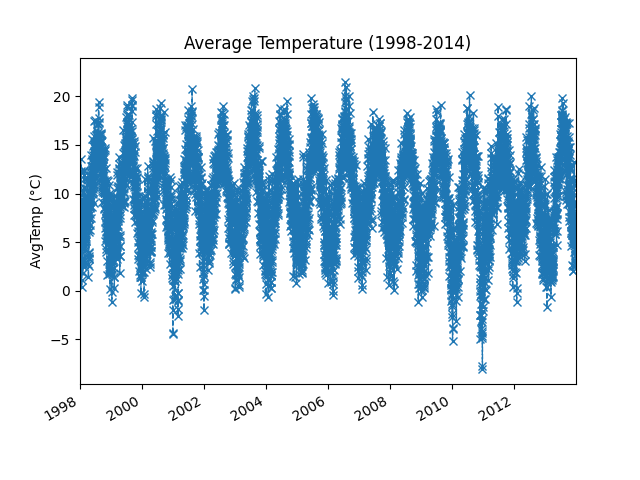
\includegraphics[width=0.45\textwidth]{Figures/Average Temperature (1998-2014) Time Series.png}
    \caption{Time Series of Daily Average Temperature in Dublin Airport in Ireland during 1998-2014.}
    \label{tempzoom}
\end{figure}

It seems that the temperatures may be normally distributed, but we will not elaborate on that with any tests. Also note that the time series is not the true measured average temperature because we combined the maximum and minimum daily temperature and in particular we averaged them using

\begin{equation}\label{avgeq}
    X_t = \frac{T^{min}_t+T^{max}_t}{2}.
\end{equation}

\subsection{Trend}

We begin the linear analysis of $X_t$ by exploring the trend. When the trend in a time series can be described by some known or estimated time function $\mu_t$ = $f(t)$ it is called deterministic trend. But when the trend can not be described by a known (parametric) function of time, showing slow changes with time but not in a decisive way, it is called stochastic trend. In this case, we notice in Figure \ref{tempzoom} that the mean of $X_t$ is (slightly) changing in seemingly random ways. 

\begin{figure}[ht]
    \centering
    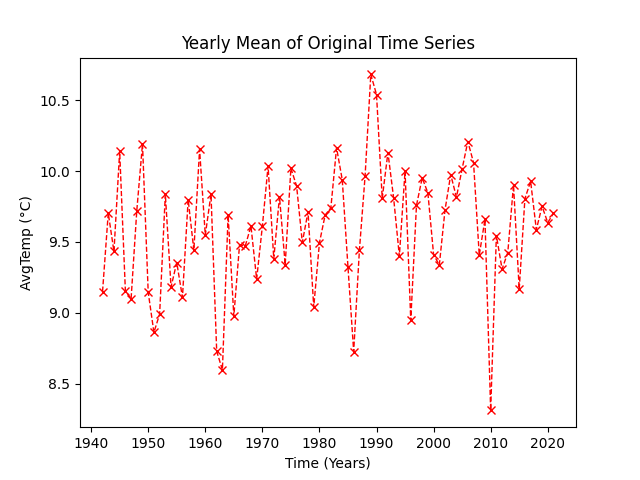
\includegraphics[width=0.45\textwidth]{Figures/Yearly Mean of Original Time Series.png}
    \caption{Yearly Mean Average Temperature.}
    \label{tempym}
\end{figure}

Also by looking at the yearly mean average temperature in Figure \ref{tempym} we can see that the mean of average temperature is changing in stochastic ways from year to year. Furthermore, by observing the autocorrelation of $X_t$ in Figure \ref{tempcf} we confirm that the time series is not stationary. We see that there is a significant correlation ($> 0.5$) between days for lag = $1$ to even lag = $40$. For these reasons we conclude that there exists a stochastic trend and we decide to eliminate it, because we believe it is produced by factors such as climate change, whereas we want to study the mechanism the temperature functions with and find the correlation between the values themselves. 

\begin{figure}[ht]
    \centering
    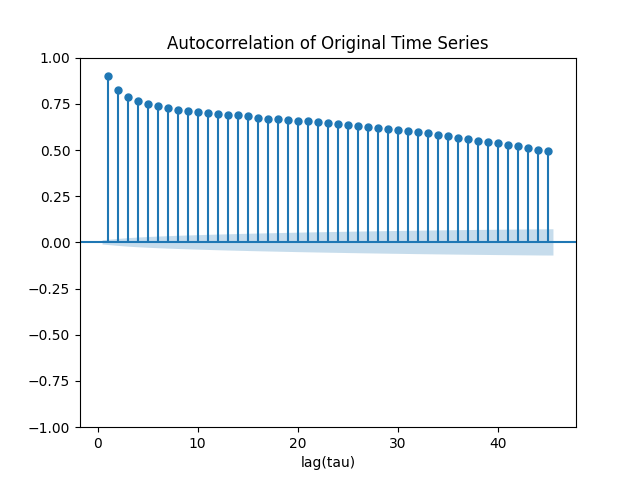
\includegraphics[width=0.45\textwidth]{Figures/Autocorrelation of Original Time Series.png}
    \caption{Autocorrelation.}
    \label{tempcf}
\end{figure}

We studied three ways of detrending $X_t$. The first is letting the possibility a deterministic trend exists and trying to estimate a polynomial (parametric) function to adapt to $X_t$ and a linear function with breakpoints to local consecutive parts of $X_t$. The degree of the polynomial we chose is $40$ and the number of breakpoints 160. The fits are demonstrated in Figure \ref{airpolbr} in increased time resolution. The results in Figure \ref{airbrpol} show that even a polynomial of degree 40 can not estimate the trend of $X_t$. The mean of the time series for both the polynomial and the linear piecewise breakpoint fit still displays variations with time. 
\vspace{10mm}

\begin{figure}[ht]
    \centering
    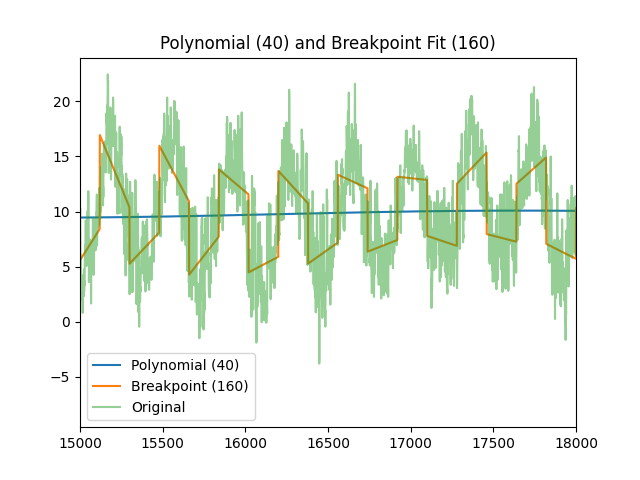
\includegraphics[width=0.45\textwidth]{Figures/Polynomial (40) and Breakpoint Fit (160).png}
    \caption{Polynomial Fit with degree $= 40$ and Linear Piecewise Fit with 160 breakpoints.}
    \label{airpolbr}
\end{figure}
\vspace{15mm}

\begin{figure}[ht]
    \centering
    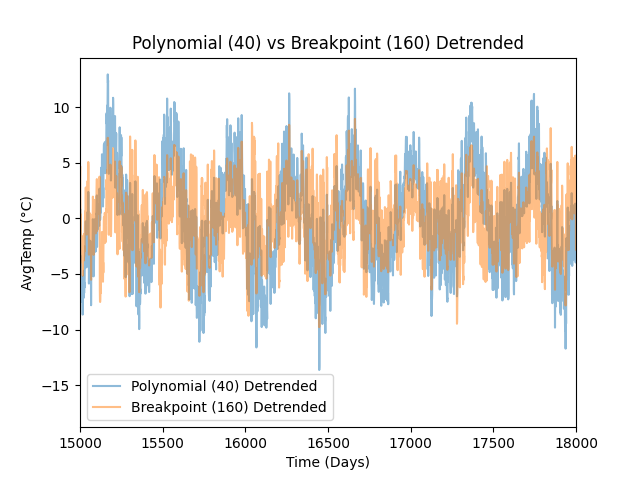
\includegraphics[width=0.45\textwidth]{Figures/Polynomial (40) vs Breakpoint (160) Detrended.png}
    \caption{Detrending $X_t$ with the polynomial and breakpoint fit.}
    \label{airbrpol}
\end{figure}
\vspace{15mm}

Proceeding with another way of detrending is by creating a moving average filter and then applying it (adapting it by taking the residuals) to $X_t$. The moving average filter we used with a window of 92 is shown in Figure \ref{airma}.
\vspace{20mm}

\begin{figure}[ht]
    \centering
    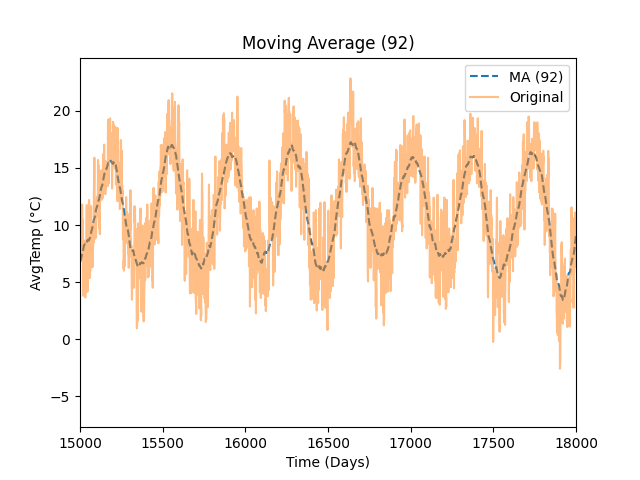
\includegraphics[width=0.45\textwidth]{Figures/Moving Average (92).png}
    \caption{Moving Average Filter with a window of 92.}
    \label{airma}
\end{figure}

Finally the last way of detrending is by obtaining the differences of logarithms of the time series by applying

\begin{equation}\label{diflog}
    \begin{split}
        & X_t^{detrended} = \nabla sign(X_t)\log|X_t| \\
        & = sign(X_t)\log|X_t|-sign(X_{t-1})\log|X_{t-1}|.
    \end{split}
\end{equation}

In Figure \ref{airfdvsma} we demonstrate the detrended time series resulting from adapting the moving average filter and applying the differences of logarithms. Judging from the figures, we concluded that it is best to detrend the time series using the moving average filter with window 92. 

\begin{figure}[ht]
    \centering
    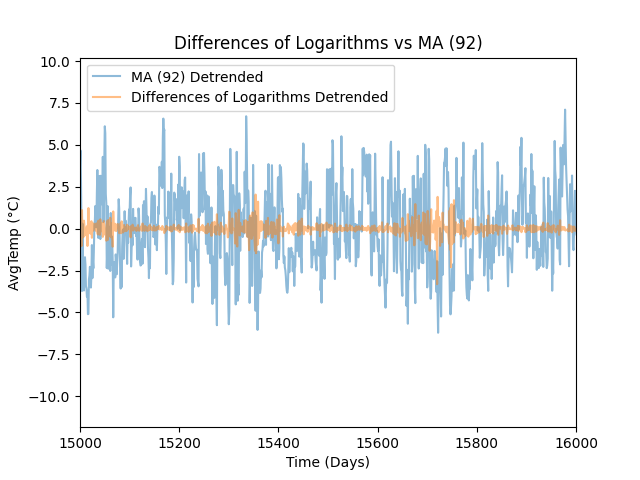
\includegraphics[width=0.45\textwidth]{Figures/Differences of Logarithms vs MA (92).png}
    \caption{Comparison of the detrended time series by adapting the moving average filter and by applying the differences of logarithms.}
    \label{airfdvsma}
\end{figure}

\subsection{Variance}

It is well known that by applying the logarithm to a time series the variance becomes invariant with time. We will check to see if this is applied to our case. In the previous section in Figure \ref{airfdvsma} we proved that the trend becomes invariant with time by using the moving average filter. This is proved in Table \ref{tablem} as the yearly means of the detrended time series are centered around zero with about $10^{-3}$ deviation which is trivial, they are practically zero. In the original time series there were clear mean fluctuations of 1 to 2 $^o C$ which is significant given that we measure temperature. 

\begin{table}
\begin{center}
\begin{tabular}{||c||c||c||} 
 \hline 
 Year & Means of $X_t$ & Means of $X_t^{detrended}$ \\ [0.5ex] 
 \hline\hline
 1942 & 9.15 & 0.17 \\ 
 \hline
 1952 & 8.86 & 0.12 \\
 \hline
 1962 & 9.55 & -0.01 \\
 \hline
 1972 & 9.24 & -0.03 \\
 \hline
 1982 & 9.71 & 0.04 \\
 \hline
 1992 & 9.44 & -0.08 \\
 \hline
 2002 & 8.95 & -0.009 \\
 \hline
 2012 & 10.02 & -0.04 \\
 \hline
 2021 & 9.9 & -0.05 \\
 \hline
\end{tabular}
\end{center}
\caption{Yearly Means of original and Detrended\break Average Temperature Time Series.}
\label{tablem}
\end{table}

The same methodology will be applied to check the variance. In Figure \ref{tempv} the yearly variance of the original time series is shown. 

\begin{figure}[ht]
    \centering
    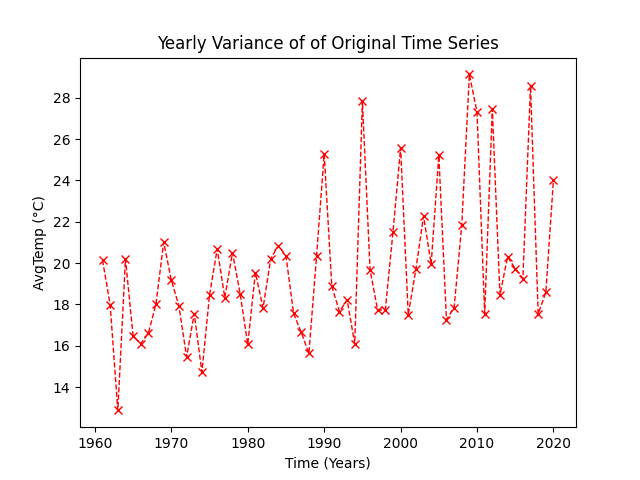
\includegraphics[width=0.45\textwidth]{Figures/Yearly Variance of of Original Time Series.png}
    \caption{Yearly Variance of original Average Temperature Time Series.}
    \label{tempv}
\end{figure}

After using the moving average filter, the yearly variance has smaller fluctuations with time. The simplest solution we applied to make the variance invariant with time is use the logarithm of the positively shifted detrended time series to produce $X_t^{final}$. The exact transformation for every observation is

\begin{equation}\label{logmas}
    \begin{split}
        & x_t^{final} = \log\left(x_t^{detrended}+\left|\min(X_t^{detrended})\right|+1\right).
    \end{split}
\end{equation}
\vspace{8mm}

The results are demonstrated in Table \ref{tablev}. The variance is now practically zero for every year. Now after centering the time series, thus subtracting the mean from every observation, We also checked to see what happened to the trend when we applied the logarithm, and as shown in Table \ref{table1m}, the mean for every year is invariant with time and centered at $0 ^o C$.

\begin{table}
\begin{center}
\begin{tabular}{||c||c||c||c||} 
 \hline 
 Year & Variances of $X_t$ & \makecell{Variances of\\$X_t^{detrended}$} & \makecell{Variances of\\$\log X_t^{detrended}$} \\ [0.5ex] 
 \hline\hline
 1950 & 19.6 & 6.4 & 0.05 \\ 
 \hline
 1959 & 21.8 & 6 & 0.06\\
 \hline
 1968 & 17.6 & 5.1 & 0.04\\
 \hline
 1977 & 24.2 & 5.3 & 0.04\\
 \hline
 1986 & 21.4 & 7.4 & 0.06\\
 \hline
 1995 & 14 & 4.7 & 0.04\\
 \hline
 2004 & 21.5 & 5.7 & 0.05\\
 \hline
 2013 & 16.7 & 6 & 0.05\\
 \hline
 2021 & 22.5 & 7.2 & 0.05\\
 \hline
\end{tabular}
\end{center}
\caption{Yearly Variance of original, detrended and logarithm \break of detrended Average Temperature Time Series.}
\label{tablev}
\end{table}

\begin{table}
\begin{center}
\begin{tabular}{||c||c||c||c||} 
 \hline 
 Year & \makecell{Mean of\\$\log X_t^{detrended}$} \\ [0.5ex]
 \hline\hline
 1950 & 0.014\\ 
 \hline
 1959 & 0.016\\
 \hline
 1968 & 0.002\\
 \hline
 1977 & -0.007\\
 \hline
 1986 & 0.003\\
 \hline
 1995 & -0.011\\
 \hline
 2004 & -0.003\\
 \hline
 2013 & -0.006\\
 \hline
 2021 & 0.0017\\
 \hline
\end{tabular}
\end{center}
\caption{Yearly Mean of logarithm of the detrended \break Average Temperature Time Series.}
\label{table1m}
\end{table}

\subsection{Seasonality}

The initial time series in Figure \ref{tempzoom} has an obvious seasonality. That makes sense because every year 
the same seasons come and go and this is basically the definition of seasons, with summer usually having the highest temperatures and winter the lowest. By looking at Figures \ref{logfin} and \ref{logfinzoom} we see that by applying the moving of average filter of order 92 the seasonality is eliminated and this is still a fact when the logarithm is applied to the whole time series.

\begin{figure}[ht]
    \centering
    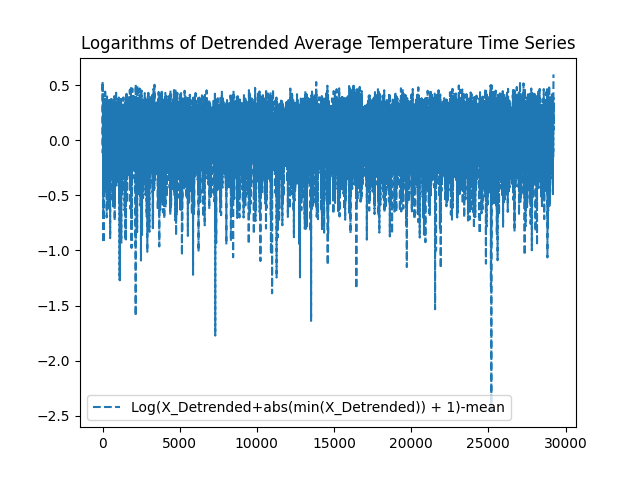
\includegraphics[width=0.45\textwidth]{Figures/Logarithms of Detrended Average Temperature Time Series.png}
    \caption{Logarithms of Detrended Average Temperature Time Series.}
    \label{logfin}
\end{figure}

\begin{figure}[ht]
    \centering
    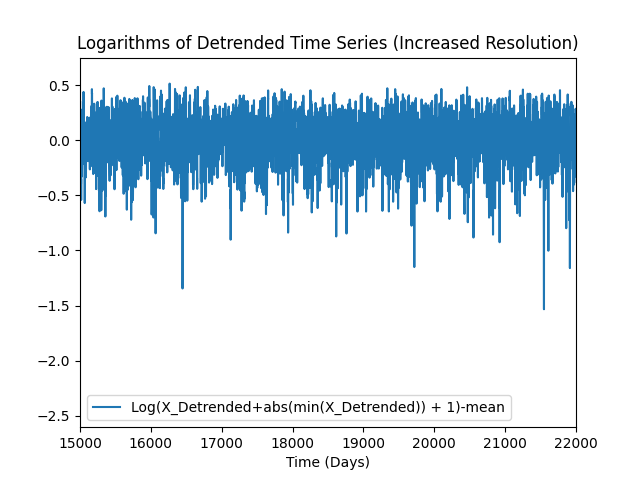
\includegraphics[width=0.45\textwidth]{Figures/Logarithms of Detrended Time Series (Increased Resolution).png}
    \caption{Logarithms of Detrended Average Temperature Time Series (Increased Resolution).}
    \label{logfinzoom}
\end{figure}

Now that we have eliminated the trend and seasonality and stabilized the variance of $X_t$ we can say that the time series is weakly stationary.

\subsection{Autocorrelation}

The autocorrelation of the detrended time series is shown in Figure \ref{airfddt} for $\tau = 31$ lags with $95\%$ confidence intervals for significant correlations. We notice that there are significant correlations that decay exponentially and become insignificant after about $\tau = 7$ lags, which is to be expected given that we analyze temperature.

\begin{figure}[ht]
    \centering
    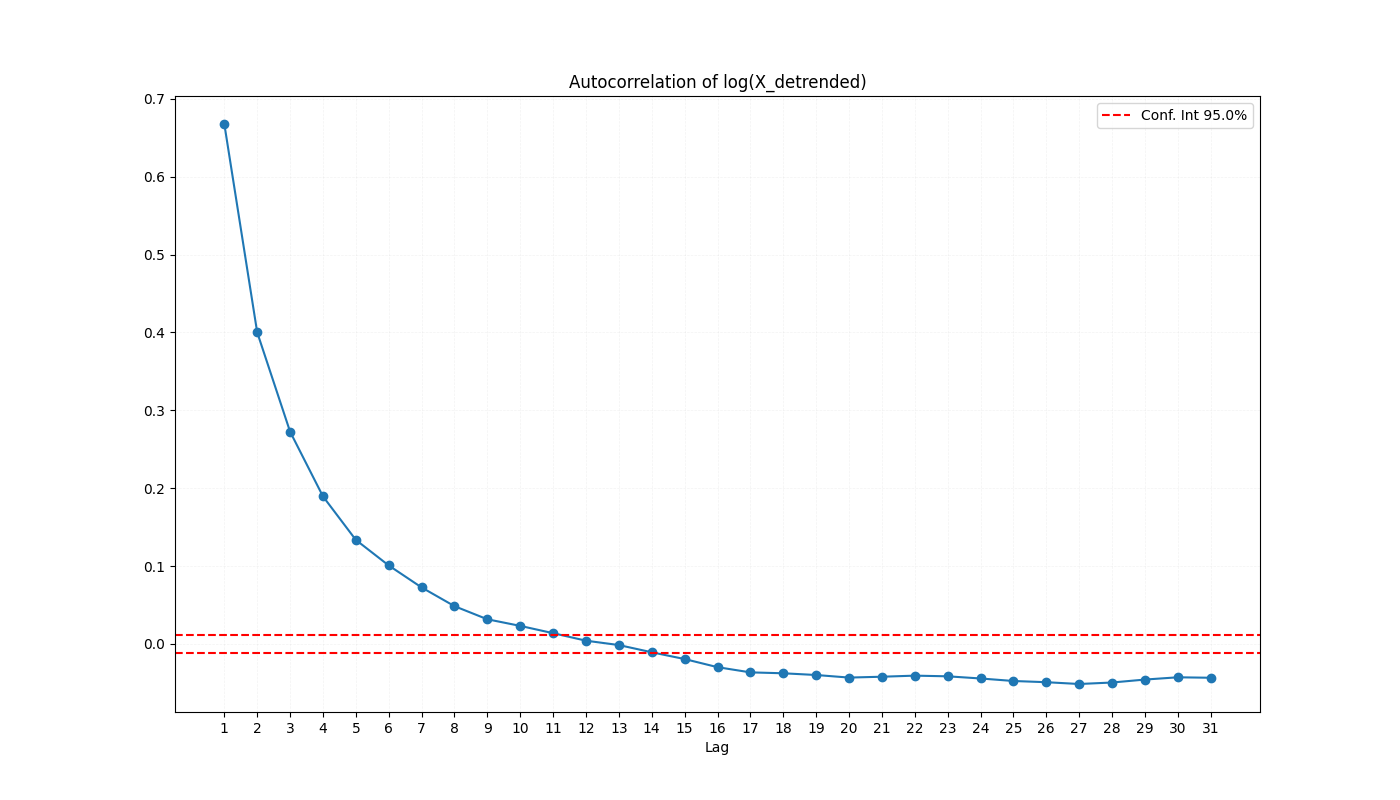
\includegraphics[width=0.45\textwidth]{Figures/Autocorrelation of log(X_detrended).png}
    \caption{Autocorrelation for the final detrended time series for $\tau = 31$ lags.}
    \label{airfddt}
\end{figure}
\vspace{7mm}

\subsection{Forecasting}

We will explore both the AR and Ma models for the time series, and also the ARMA. By calculating the partial autocorrelation we can see what $p$ to use for $AR(p)$. The partial autocorrelation is shown in Figure \ref{airfddts}. Also judging by the Akaike Information Criterion, we choose an AR model of order $6$ $(AR(6))$. The fit of this model, as well as the residuals, to the time series is shown in Figure \ref{ar6}.
\vspace{7mm}

\begin{figure}[ht]
    \centering
    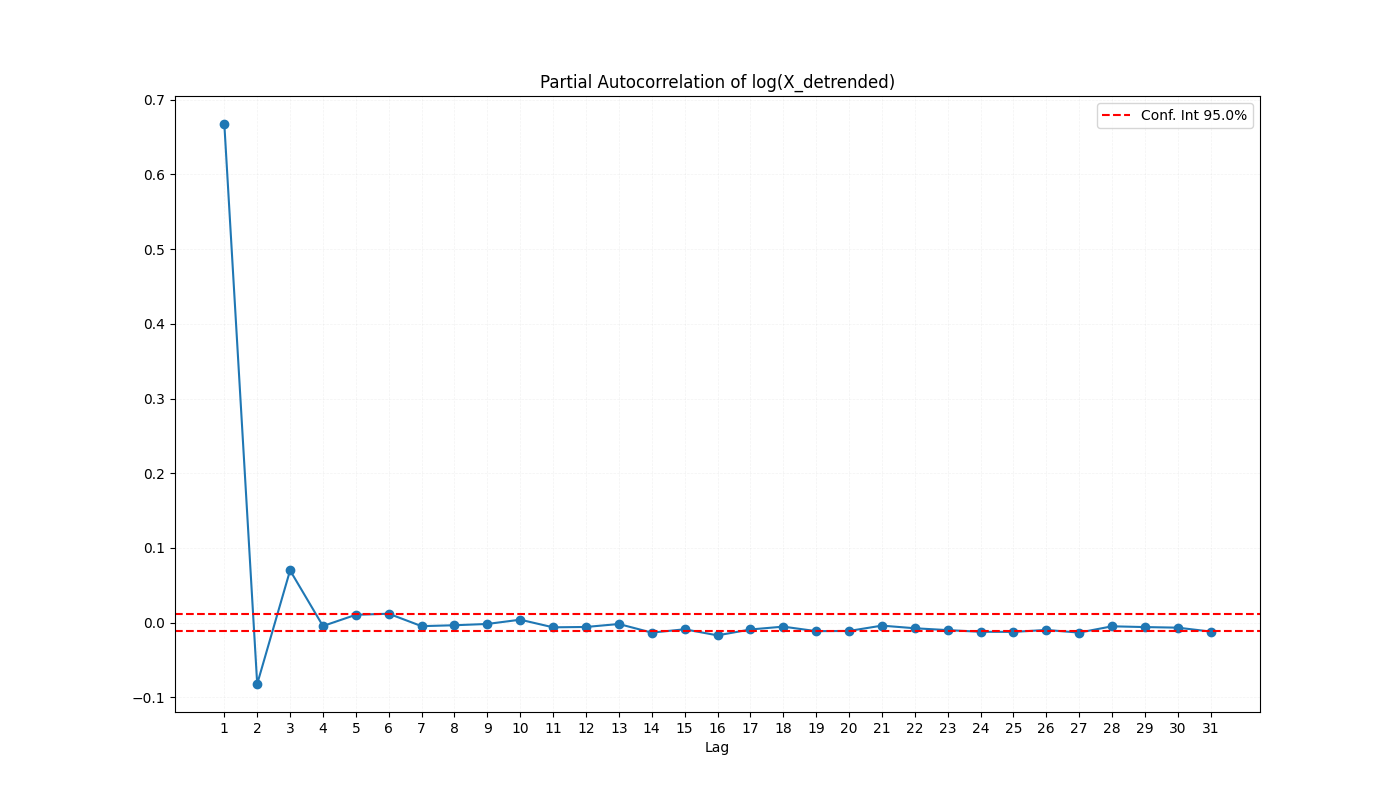
\includegraphics[width=0.45\textwidth]{Figures/Partial Autocorrelation of log(X_detrended).png}
    \caption{Partial Autocorrelation for the final detrended time series for $\tau = 31$ lags.}
    \label{airfddts}
\end{figure}

\begin{figure}[ht]
    \centering
    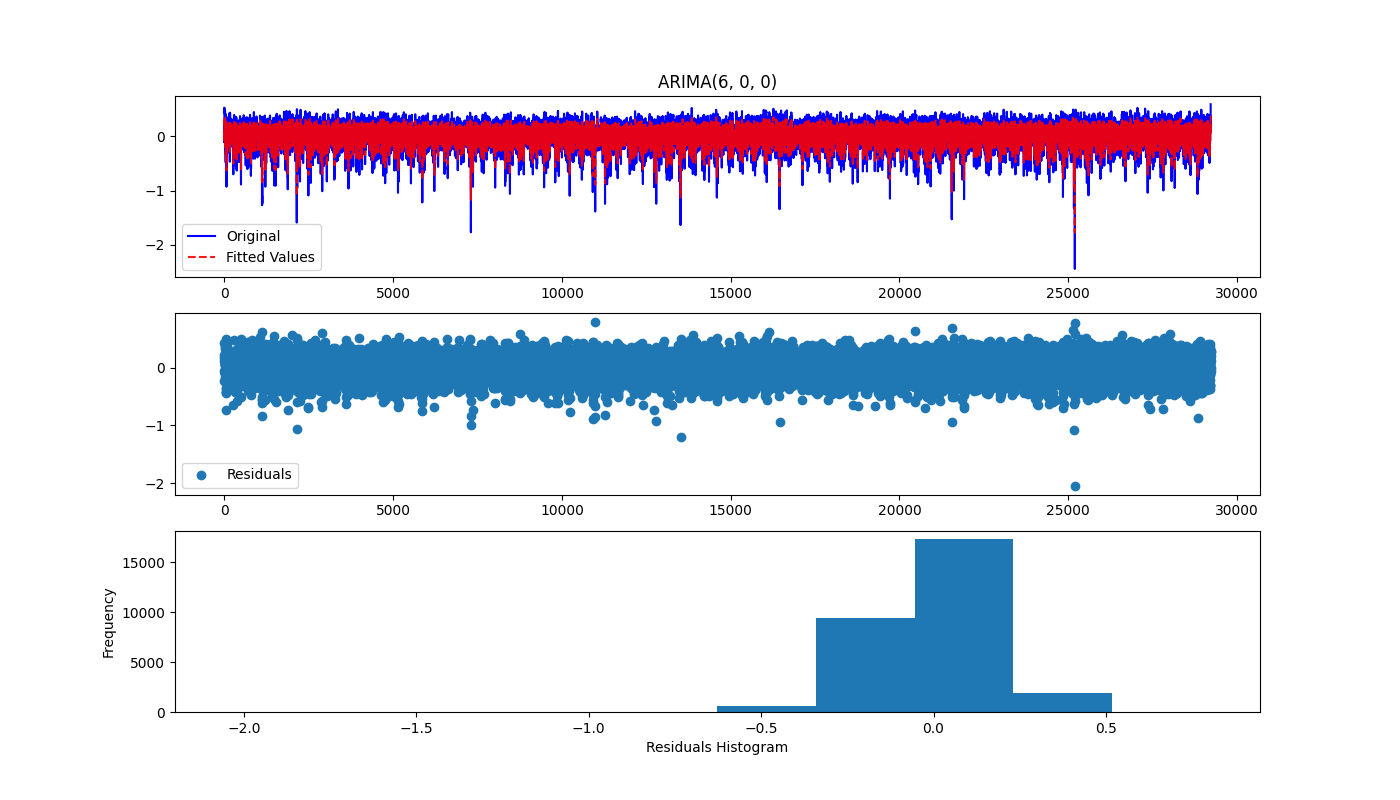
\includegraphics[width=0.45\textwidth]{Figures/ARIMA(6,0,0).png}
    \caption{AR(6) model fit to the the time series.}
    \label{ar6}
\end{figure}

The fitting error for T=10 is demonstrated in Figure \ref{fe6}. We can see that the AR(6) achieves a very good fit to the time series. The out of sample predictions of the model for time horizon T=36 and the rolling out of sample predictions for one year are shown in Figures \ref{hor6} and \ref{rol6}. We can see that the rolling predictions make a very good fit to the time series. 

\begin{figure}[ht]
    \centering
    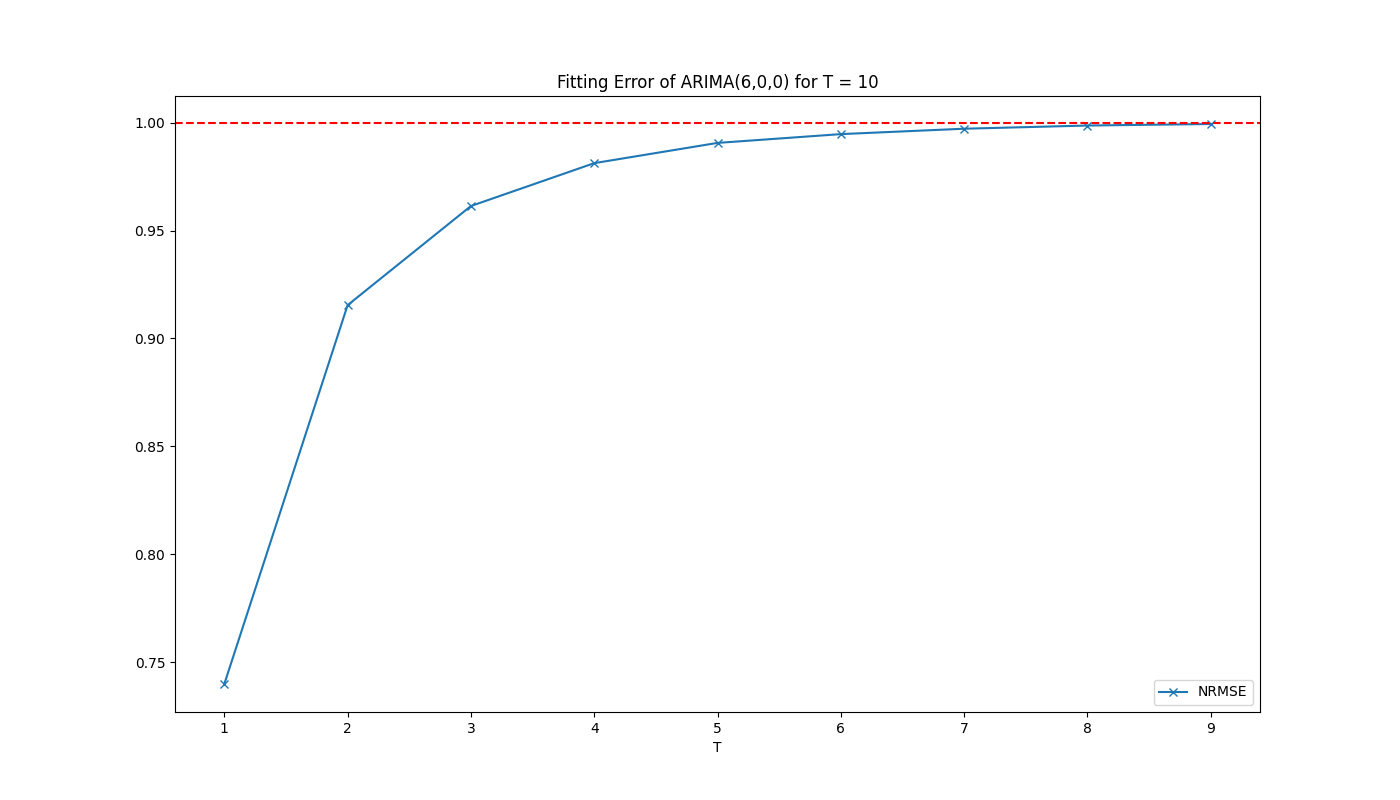
\includegraphics[width=0.45\textwidth]{Figures/Fitting Error of ARIMA(6,0,0) for T = 10.png}
    \caption{AR(6) fitting error for T=10.}
    \label{fe6}
\end{figure}

\begin{figure}[ht]
    \centering
    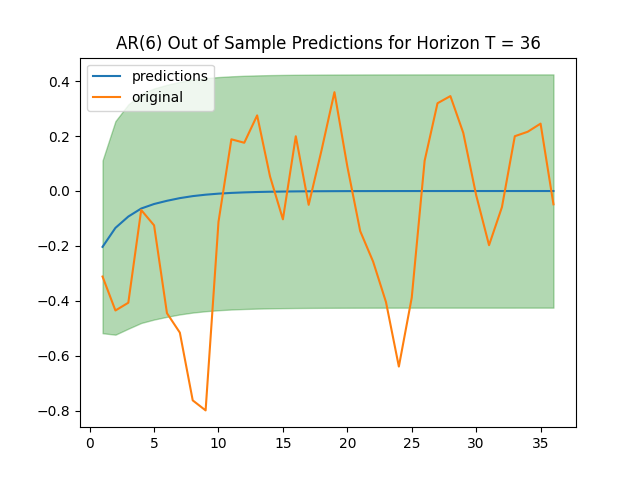
\includegraphics[width=0.45\textwidth]{Figures/AR(6) Out of Sample Predictions for Horizon T = 36.png}
    \caption{AR(6) Out of Sample Predictions for Horizon T = 36.}
    \label{hor6}
\end{figure}

\begin{figure}[ht]
    \centering
    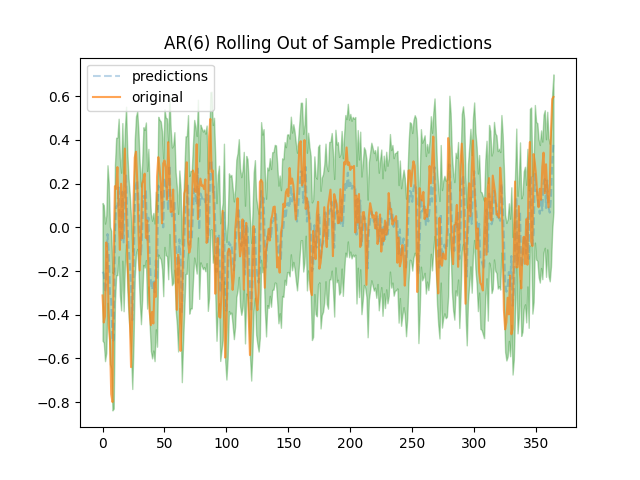
\includegraphics[width=0.45\textwidth]{Figures/AR(6) Rolling Out of Sample Predictions.png}
    \caption{AR(6) Rolling Out of Sample Predictions for one year.}
    \label{rol6}
\end{figure}
\vspace{30mm}

By exploring the MA and ARMA models we get the results shown in Figures \ref{ma9} - \ref{rol33}. The same procedure (AIC) was followed to select their orders. We can also see that the models MA(9) and ARMA(3,3) also achieve great fits. We chose AR(6) as our model-to-go, as we feel it expresses the temperature time series more accurately.

\begin{figure}[ht]
    \centering
    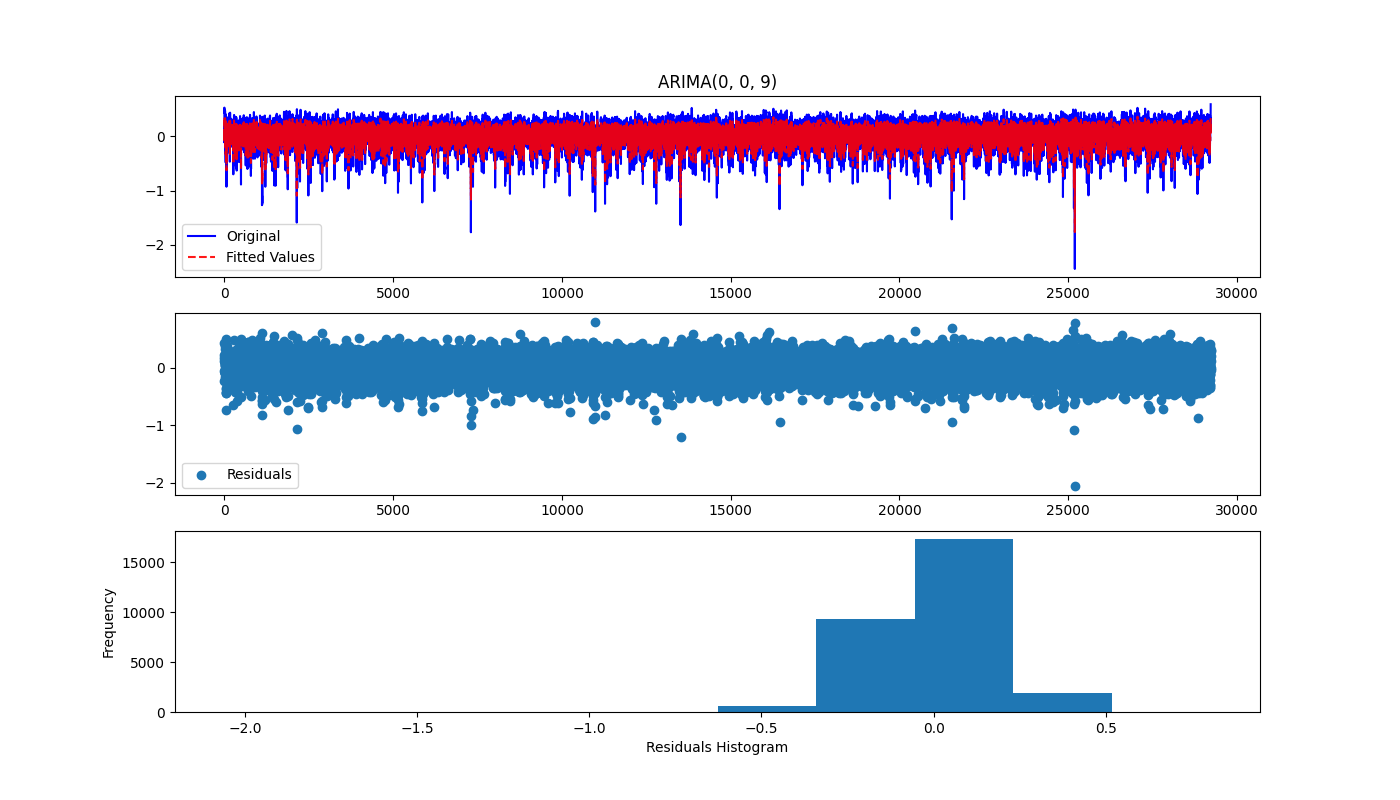
\includegraphics[width=0.45\textwidth]{Figures/ARIMA(0,0,9).png}
    \caption{MA(9) model fit to the the time series.}
    \label{ma9}
\end{figure}

\begin{figure}[ht]
    \centering
    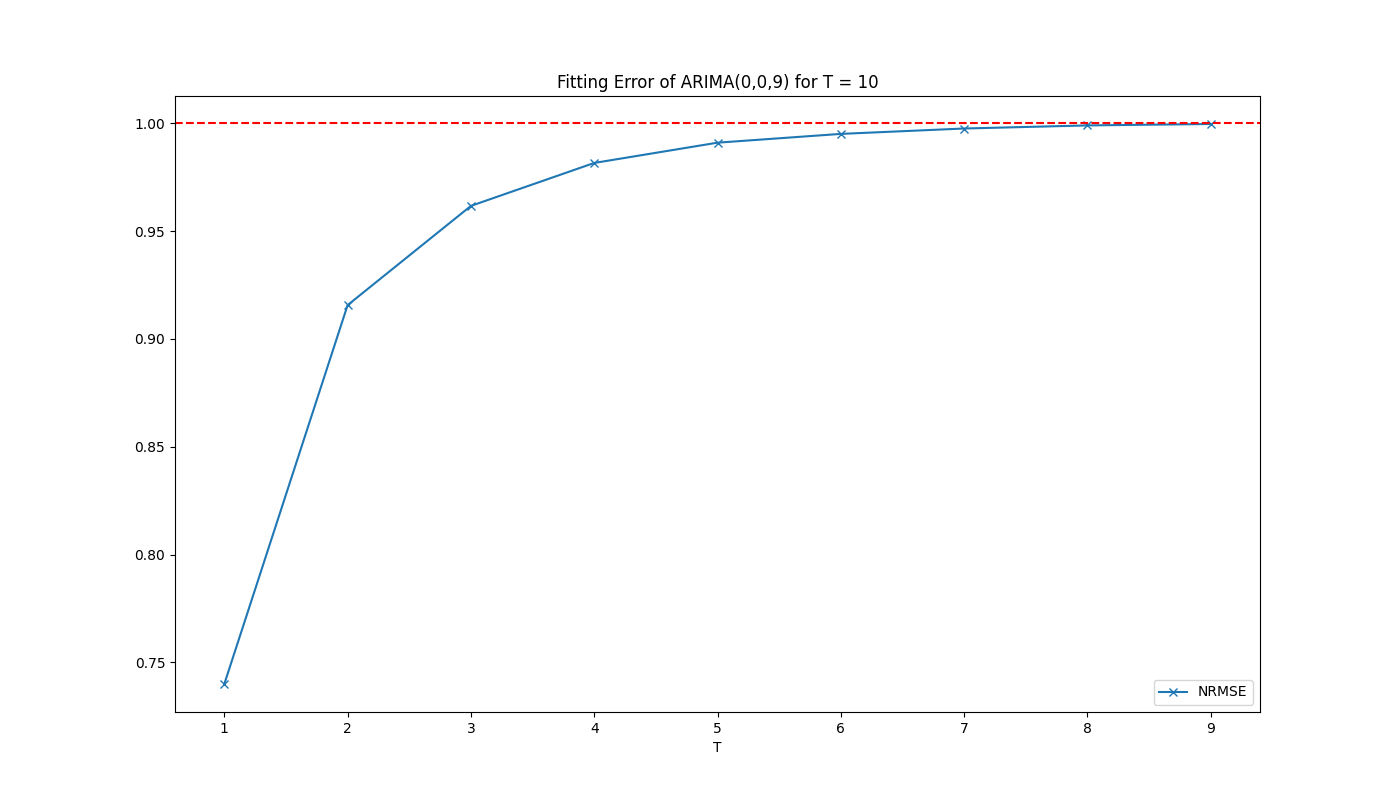
\includegraphics[width=0.45\textwidth]{Figures/Fitting Error of ARIMA(0,0,9) for T = 10.png}
    \caption{MA(9) fitting error for T=10.}
    \label{fe9}
\end{figure}

\begin{figure}[ht]
    \centering
    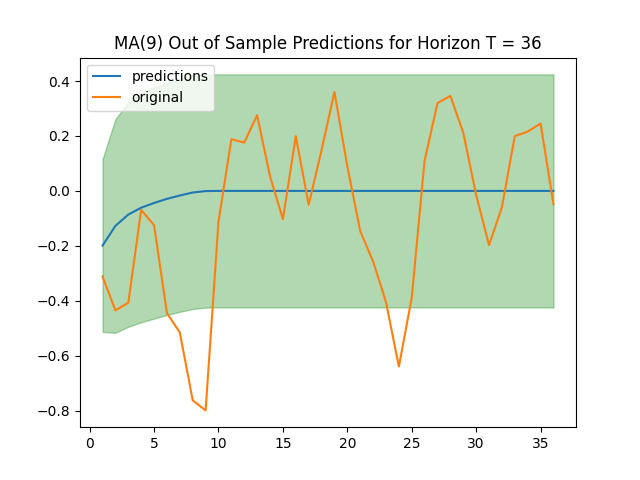
\includegraphics[width=0.45\textwidth]{Figures/MA(9) Out of Sample Predictions for Horizon T = 36.png}
    \caption{MA(9) Out of Sample Predictions for Horizon T = 36.}
    \label{hor9}
\end{figure}
\vspace{40mm}

\begin{figure}[ht]
    \centering
    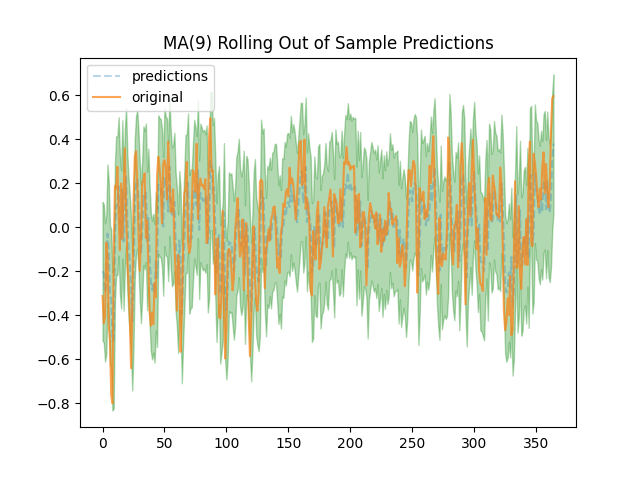
\includegraphics[width=0.45\textwidth]{Figures/MA(9) Rolling Out of Sample Predictions.png}
    \caption{MA(9) Rolling Out of Sample Predictions for one year.}
    \label{rol9}
\end{figure}
\vspace{30mm}

\begin{figure}[ht]
    \centering
    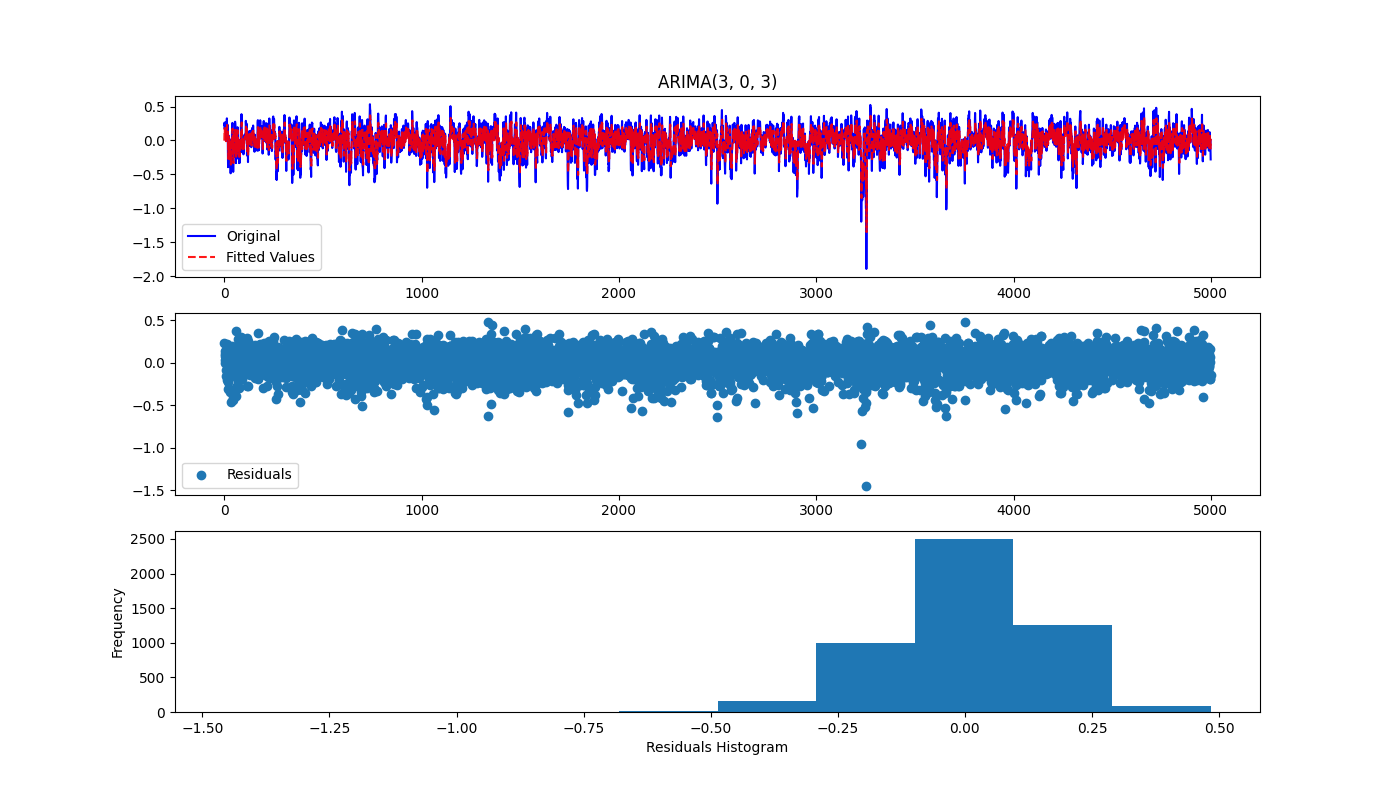
\includegraphics[width=0.45\textwidth]{Figures/ARIMA(3,0,3).png}
    \caption{ARMA(3,3) model fit to the the time series.}
    \label{ma33}
\end{figure}

\begin{figure}[ht]
    \centering
    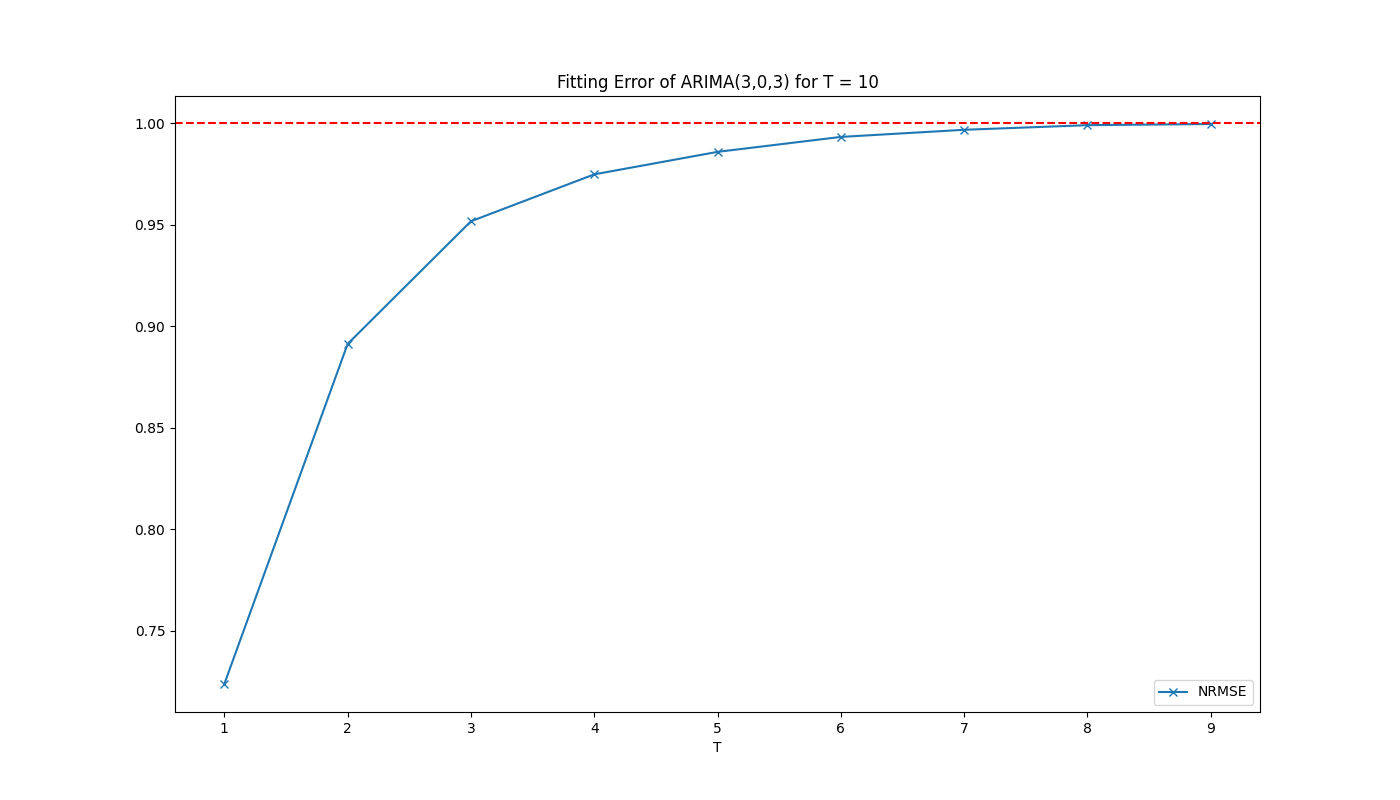
\includegraphics[width=0.45\textwidth]{Figures/Fitting Error of ARIMA(3,0,3) for T = 10.png}
    \caption{ARMA(3,3) fitting error for T=10.}
    \label{fe33}
\end{figure}

\begin{figure}[ht]
    \centering
    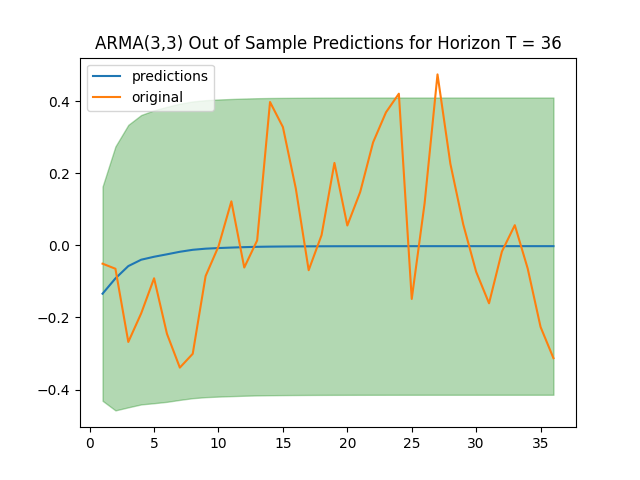
\includegraphics[width=0.45\textwidth]{Figures/ARMA(3,3) Out of Sample Predictions for Horizon T = 36.png}
    \caption{ARMA(3,3) Out of Sample Predictions for Horizon T = 36.}
    \label{hor33}
\end{figure}
\vspace{40mm}

\begin{figure}[ht]
    \centering
    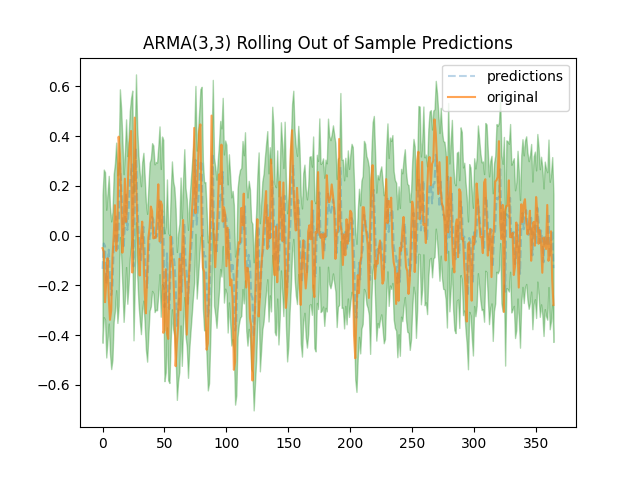
\includegraphics[width=0.45\textwidth]{Figures/ARMA(3,3) Rolling Out of Sample Predictions.png}
    \caption{ARMA(3,3) Rolling Out of Sample Predictions for one year.}
    \label{rol33}
\end{figure}

Finally, the Portmanteau tests were run for the three models, and we can see that all of them catch the linear correlations. The results are shown in Figures \ref{p6} - \ref{p33}, with AR(6) leading the way.

\begin{figure}[ht]
    \centering
    \includegraphics[width=0.40\textwidth]{Figures/Ljung-Box Portmanteau Test for Residuals of ARIMA(6,0,0).png}
    \caption{Ljung-Box Portmanteau Test for Residuals of AR(6).}
    \label{p6}
\end{figure}

\begin{figure}[ht]
    \centering
    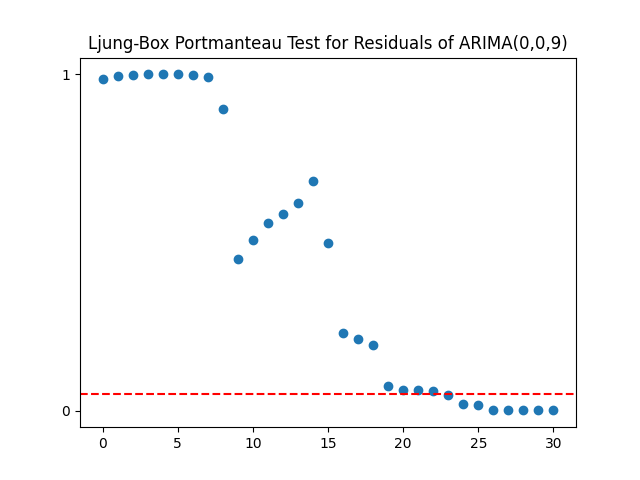
\includegraphics[width=0.40\textwidth]{Figures/Ljung-Box Portmanteau Test for Residuals of ARIMA(0,0,9).png}
    \caption{Ljung-Box Portmanteau Test for Residuals of MA(9).}
    \label{p9}
\end{figure}

\begin{figure}[ht]
    \centering
    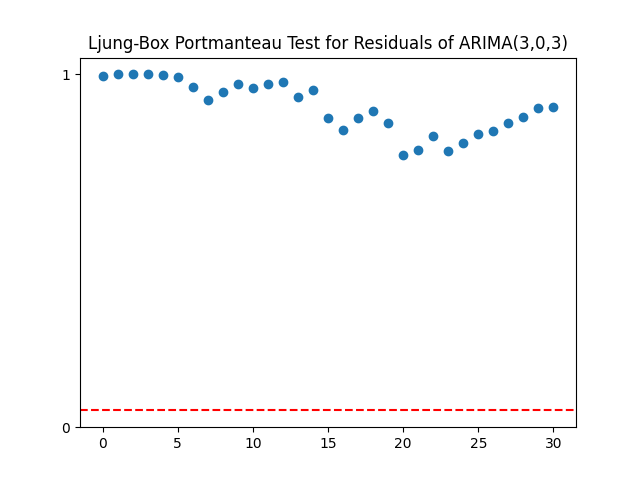
\includegraphics[width=0.45\textwidth]{Figures/Ljung-Box Portmanteau Test for Residuals of ARIMA(3,0,3).png}
    \caption{Ljung-Box Portmanteau Test for Residuals of ARMA(3,3).}
    \label{p33}
\end{figure}

%-Dublin-Airport-Average-Temperature-Non-Linear-Analysis---------------------------------------------------------
\section{Dublin Airport Average Temperature \break Non-Linear Analysis}

After testing the residuals (Figure \ref{resa}) of the stationary time series by applying the AR(6) model, we found out that they were white noise with the Portmanteau test (Figure \ref{porta}).

\begin{figure}[ht]
    \centering
    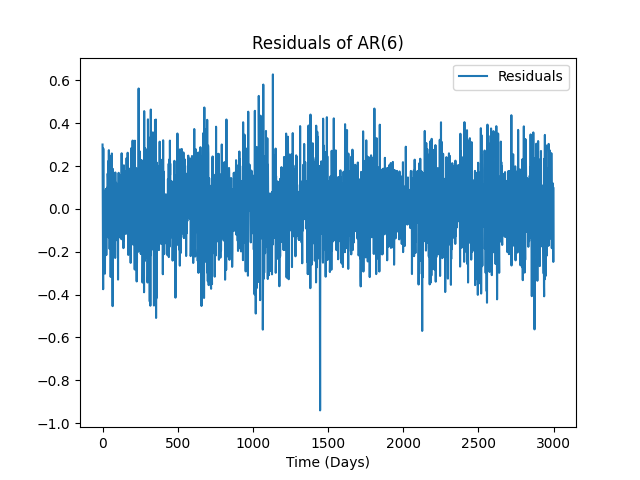
\includegraphics[width=0.40\textwidth]{Figures/AirportNonLin/Residuals of AR(6).png}
    \caption{Residuals of selected AR(6) from Linear Analysis.}
    \label{resa}
\end{figure}

\begin{figure}[ht]
    \centering
    \includegraphics[width=0.40\textwidth]{Figures/AirportNonLin/Ljung-Box Portmanteau Test for Residuals of ARIMA(6,0,0).png}
    \caption{Ljung-Box Portmanteau Test for Residuals of AR(6).}
    \label{porta}
\end{figure}

So this the time series that we are going to apply non-linear analysis to. We created 40 new time series of the same length with the original residuals, without correlations, with random permutations. This was done to explore if there are any non-linear correlations. The residuals may be white noise, but are they iid, or have they non-linear correlations? To have non-linear correlations, a statistic must have a little difference in the original residuals in respect to the 40 time series. If a statistic is linear, then the estimated statistic of the original residual time series belongs in the distribution of the statistics from the 40 time series. The first statistic that we checked for is the Dickey-Fuller stationarity Statistical Test. If the p-value of the statistic is below the significance level, the zero hypothesis ($H_0$) is rejected and the time series is stationary.

\begin{figure}[ht]
    \centering
    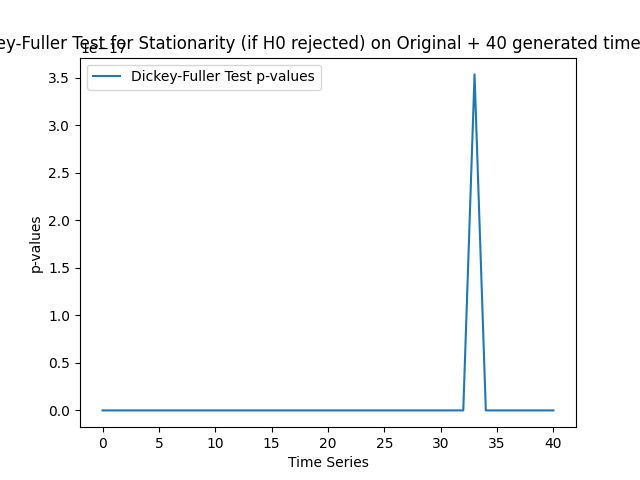
\includegraphics[width=0.45\textwidth]{Figures/AirportNonLin/Dickey-Fuller Test for Stationarity (if H0 rejected) on Original + 40 generated time series.png}
    \caption{Dickey-Fuller Test for Stationarity (if H0 rejected) on Original + 40 generated time series (y axis is scaled in $10^{-30}$).}
    \label{adfa}
\end{figure}

We can see in Figure \ref{adfa} that the zero hypothesis is rejected for the original residuals and all 40 randomly permutated time series. Subsequently, we explored the autocorrelation and the delayed mutual information for all 41 time series. The results are shown in Figures \ref{dela} and \ref{mia}. 

\begin{figure}[ht]
    \centering
    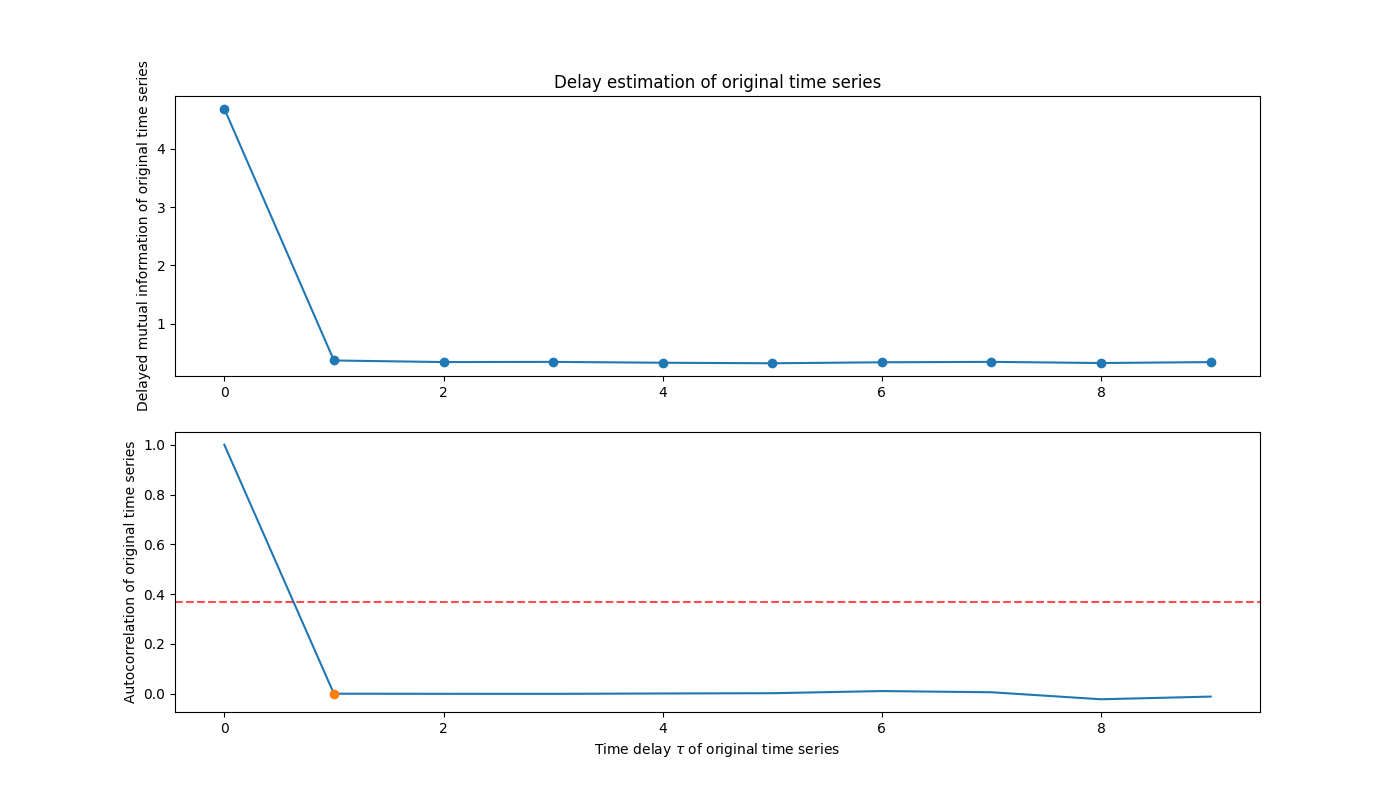
\includegraphics[width=0.45\textwidth]{Figures/AirportNonLin/Delay estimation of original time series.png}
    \caption{Delay estimation of original time series.}
    \label{dela}
\end{figure}

\begin{figure}[ht]
    \centering
    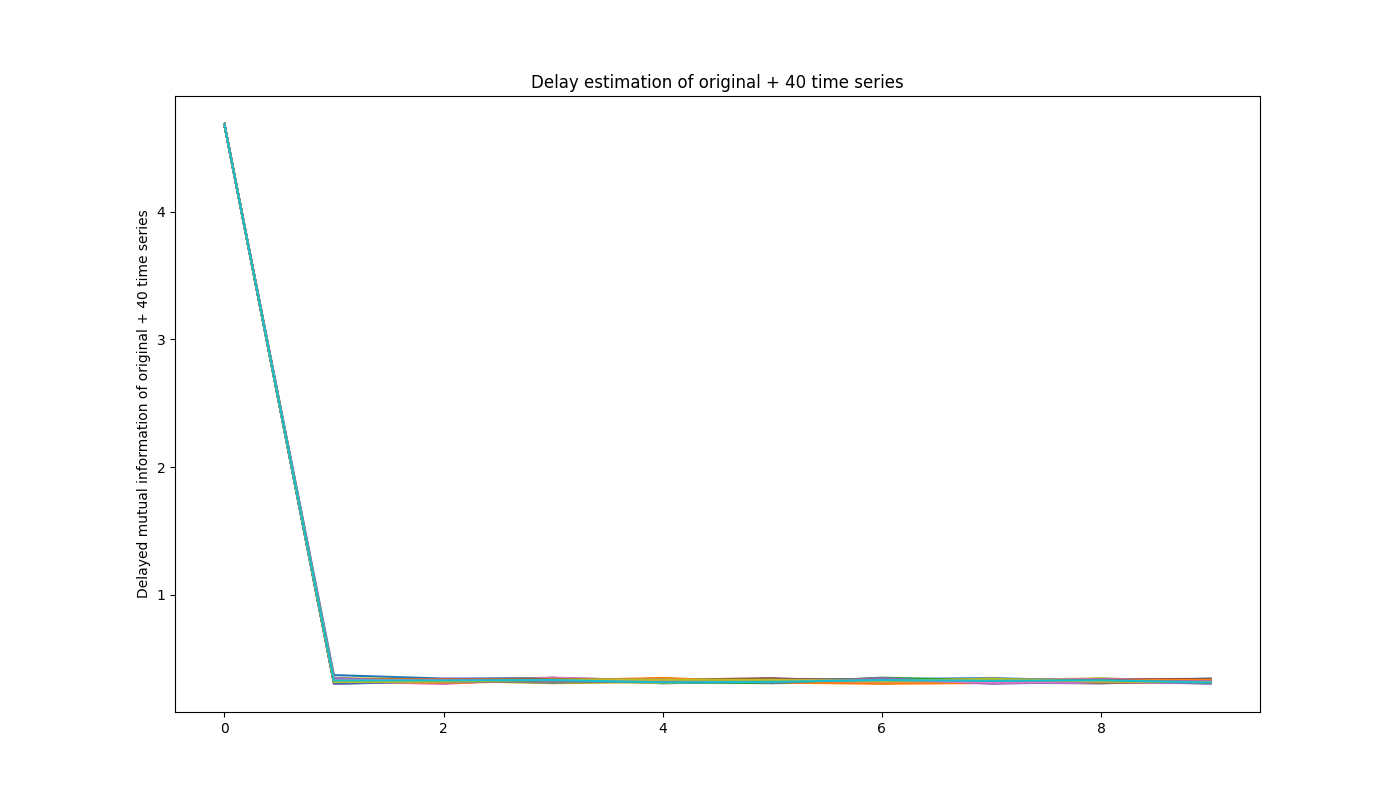
\includegraphics[width=0.45\textwidth]{Figures/AirportNonLin/Delay estimation of original + 40 time series.png}
    \caption{Delayed mutual information of original + 40 time series.}
    \label{mia}
\end{figure}

We can see that for all 41 time series the first minimum $\tau$ is one. Next we evaluated the dimension for the original and all sample time series, using the false nearest neighbors method. Figures \ref{dima} and \ref{dimalla} demonstrate the results. We notice as well that the FNN belongs in the same distribution with the 40 time series.

\begin{figure}[ht]
    \centering
    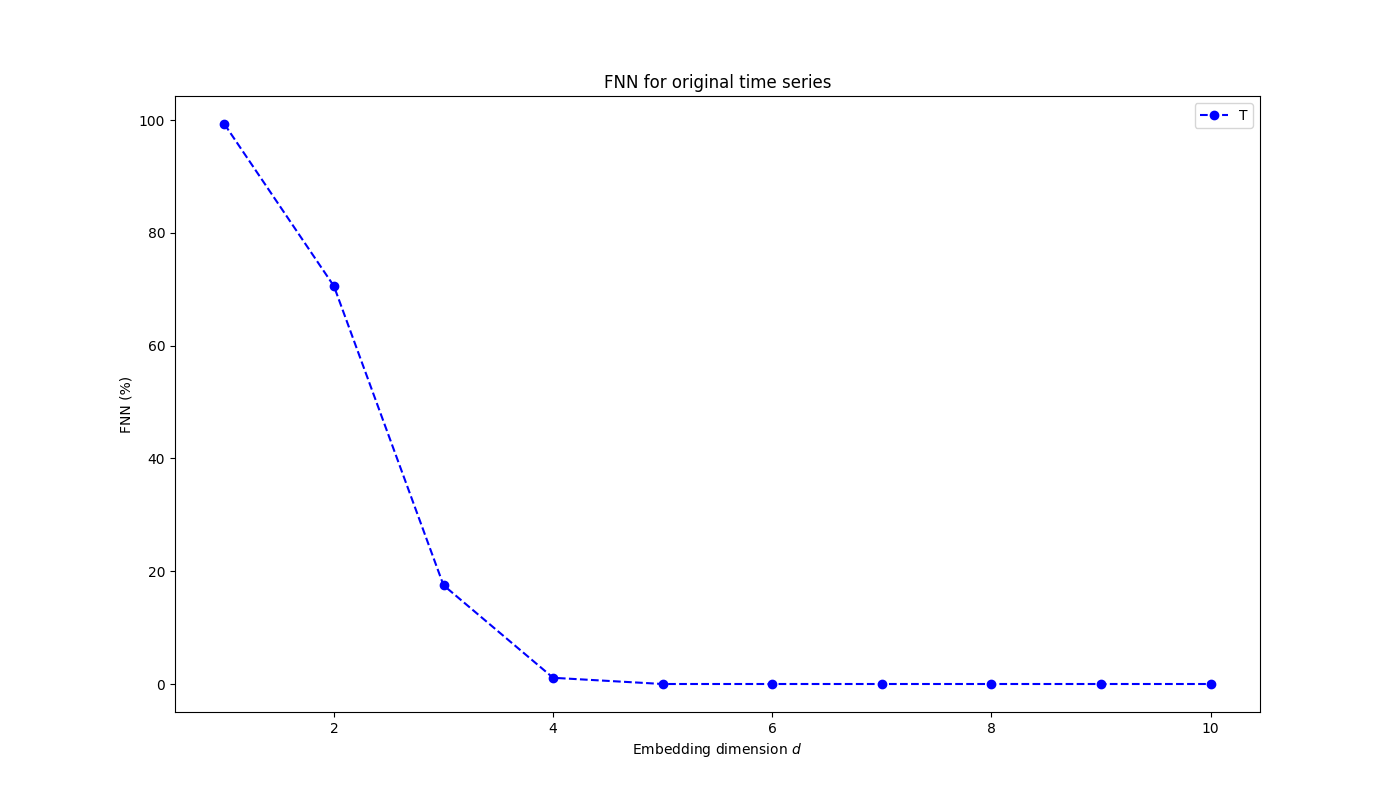
\includegraphics[width=0.45\textwidth]{Figures/AirportNonLin/FNN for original time series.png}
    \caption{False Nearest Neighbors for original time series.}
    \label{dima}
\end{figure}

\begin{figure}[ht]
    \centering
    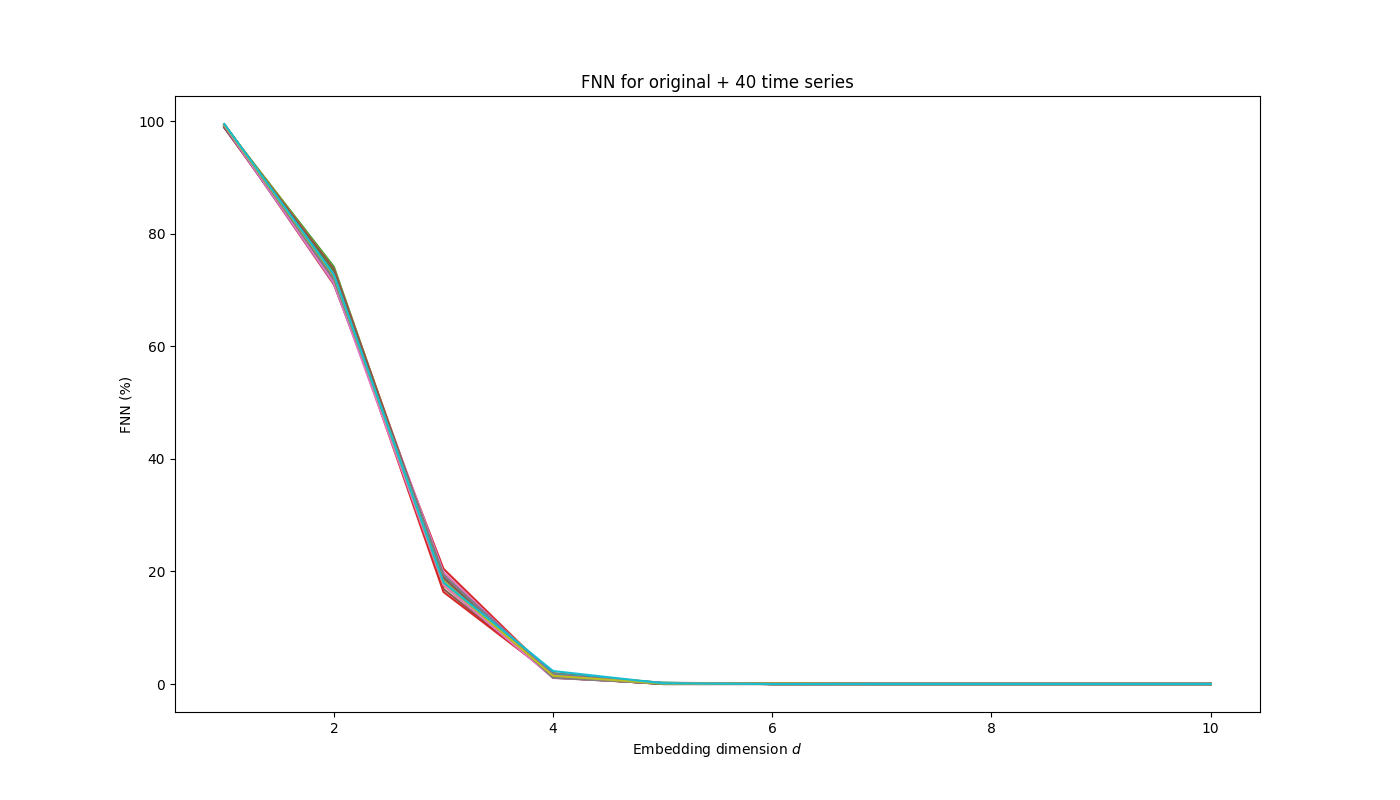
\includegraphics[width=0.45\textwidth]{Figures/AirportNonLin/FNN for original + 40 time series.png}
    \caption{False Nearest Neighbors for original + 40 time series.}
    \label{dimalla}
\end{figure}
\vspace{8mm}

Moving on, the correlation sum is shown in Figures \ref{corsuma} and \ref{corloga}.
\vspace{20mm}

\begin{figure}[ht]
    \centering
    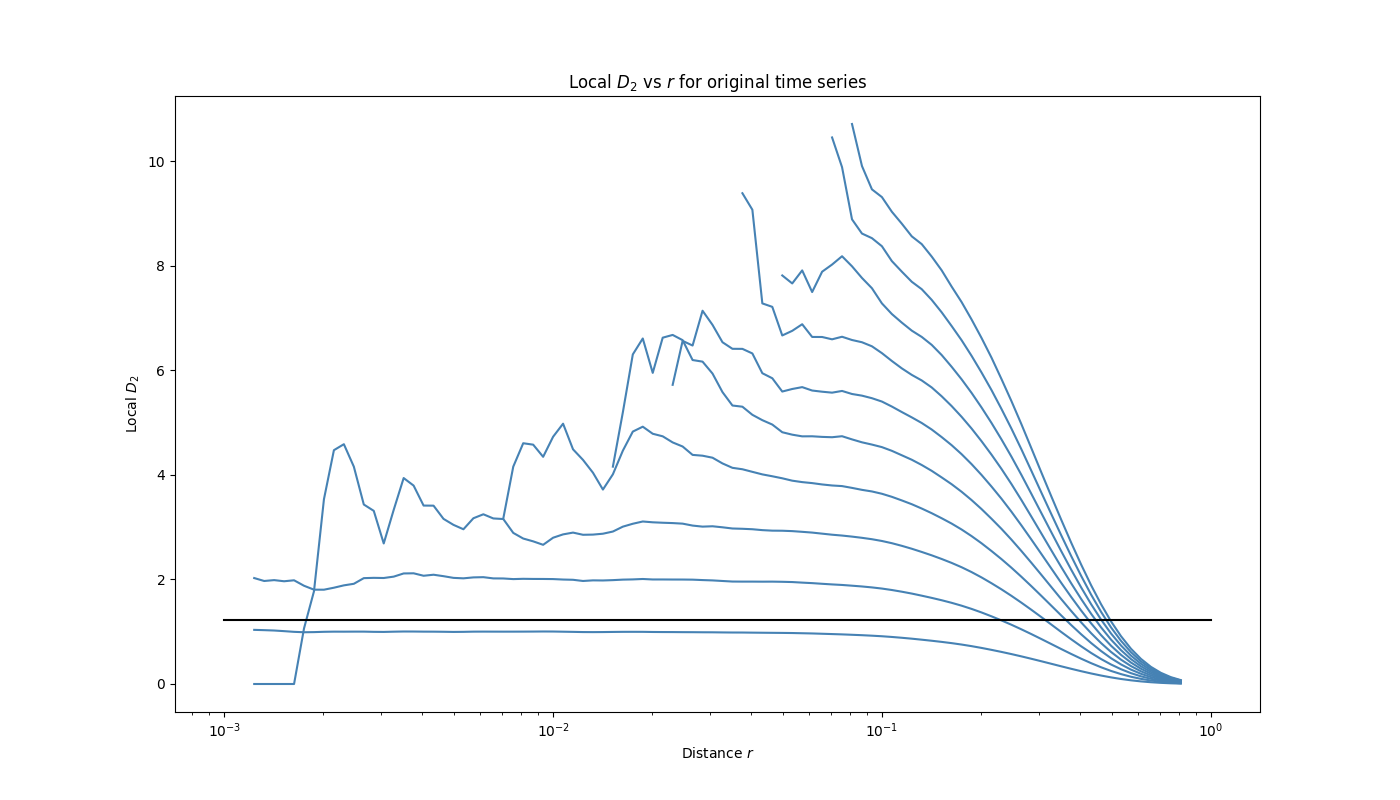
\includegraphics[width=0.45\textwidth]{Figures/AirportNonLin/Local vs for original time series.png}
    \caption{Local $D_2$ vs $r$ for original time series.}
    \label{corsuma}
\end{figure}

\begin{figure}[ht]
    \centering
    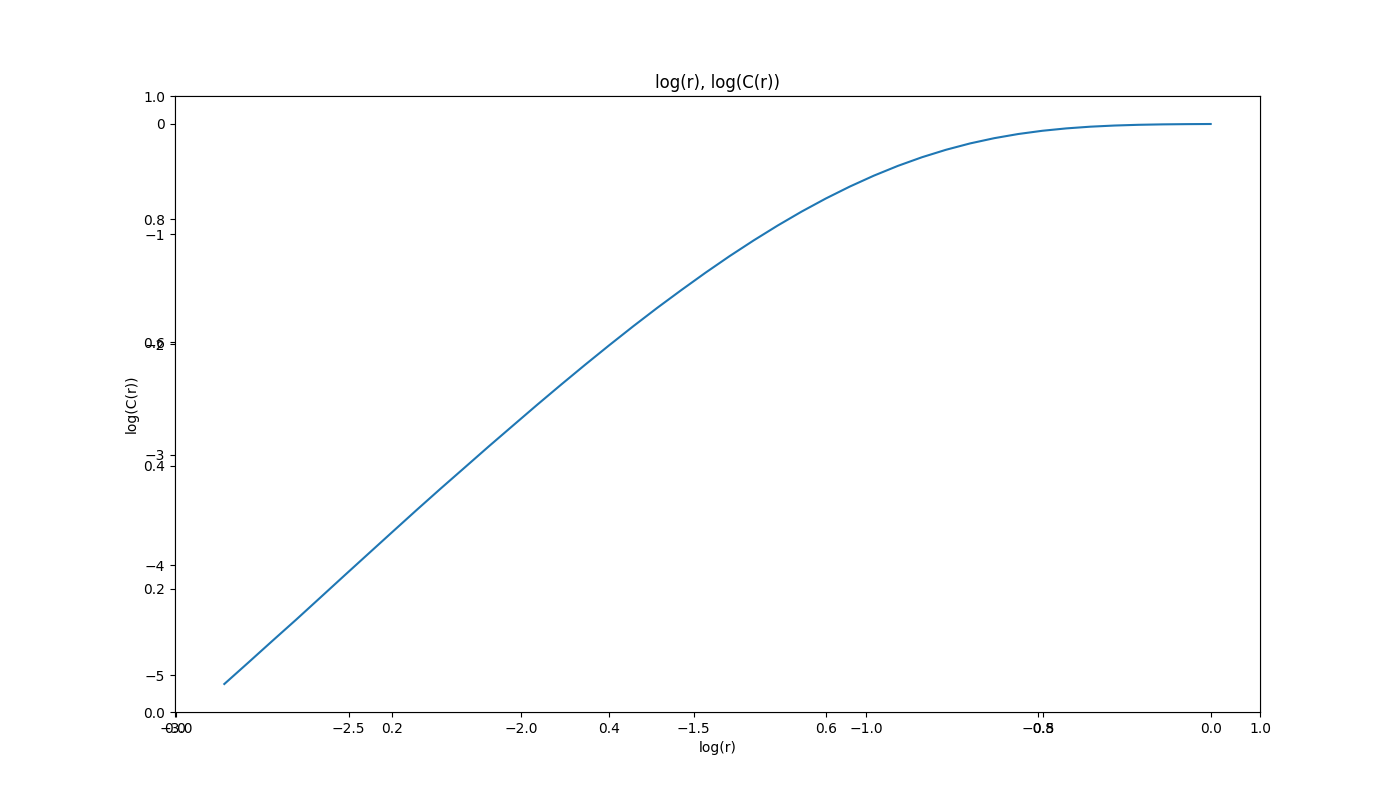
\includegraphics[width=0.45\textwidth]{Figures/AirportNonLin/log(r), log(C(r)).png}
    \caption{log(r) log(C(r)).}
    \label{corloga}
\end{figure}

Next, for embedding dimension $m = 3$ (we did not choose $m = 4$ for visualization) and $\tau = 1$ the plotted 3D Attractor is shown in Figure \ref{atta}. The attractor shape is like a cloud, implying that there is not any non-linear correlation in the time series. This was also made clear before, as the statistics that we estimated all belong to the same distribution. 

\begin{figure}[ht]
    \centering
    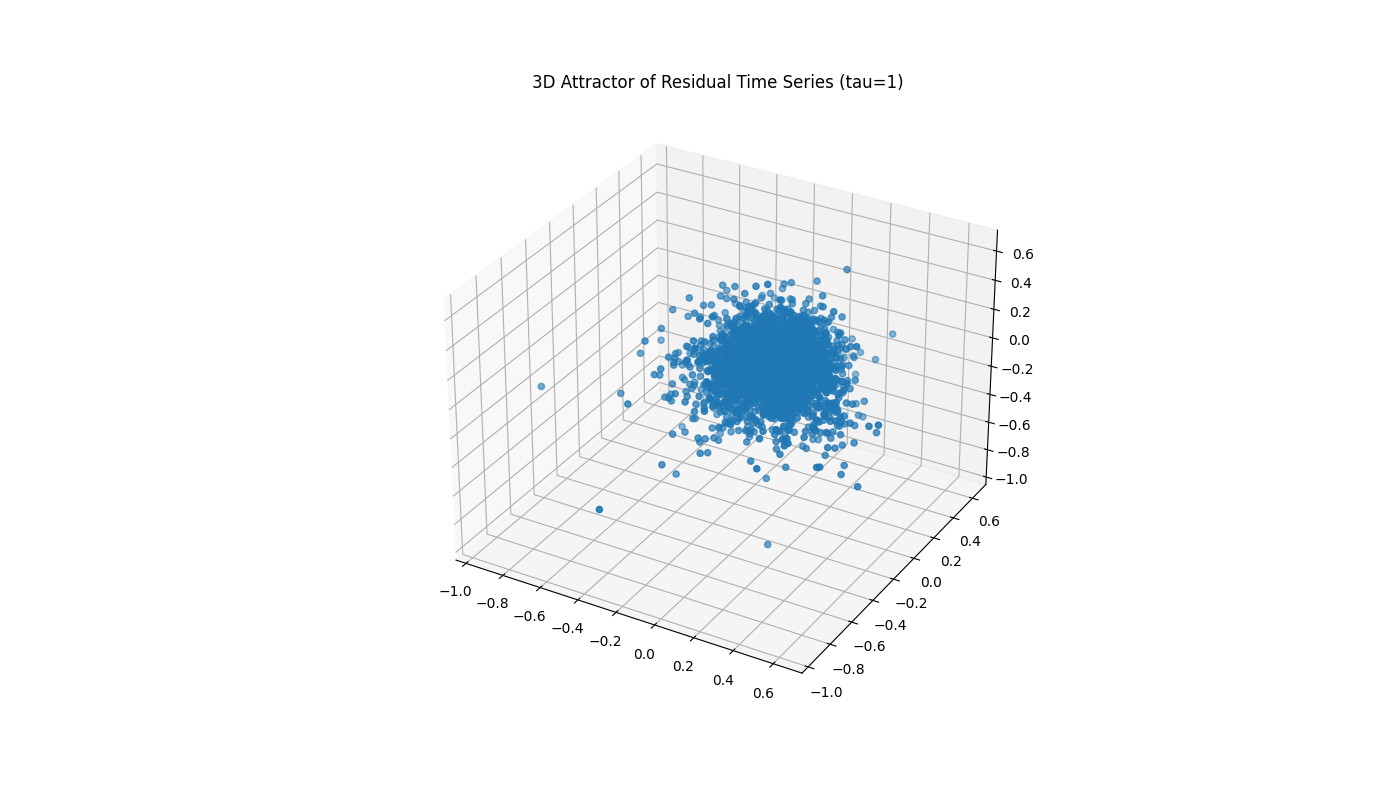
\includegraphics[width=0.45\textwidth]{Figures/AirportNonLin/3D Attractor of Residual Time Series (tau=1).png}
    \caption{3D Attractor of Residual Time Series (tau=1).}
    \label{atta}
\end{figure}

Next we explored the predictions with LAP and LLP. First of all, the train and test set are shown in Figure \ref{tra}.
\vspace{30mm}

\begin{figure}[ht]
    \centering
    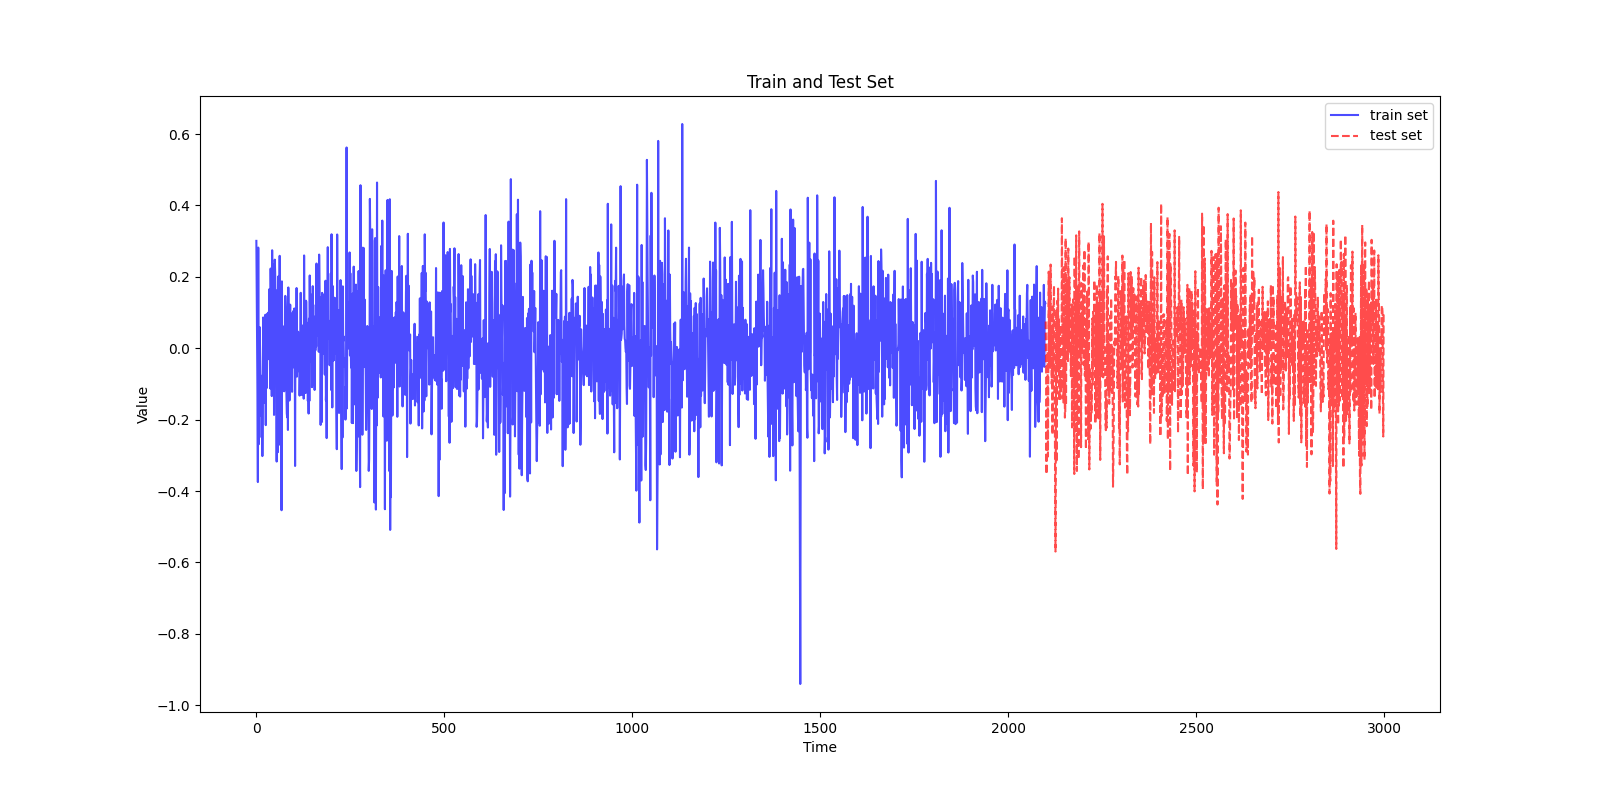
\includegraphics[width=0.40\textwidth]{Figures/AirportNonLin/Train and Test Set.png}
    \caption{Train and Test Sets.}
    \label{tra}
\end{figure}

After embedding the train and test sets in dimension 3 and $\tau = 1$, we used the KDTree. The neighbors of the first test datapoint are demonstrated in Figure \ref{ndata}, the Test Set State is shown in Figure \ref{TESTA}, and the neighbors of the first test datapoint in train data are shown in Figure \ref{traina}.

\begin{figure}[ht]
    \centering
    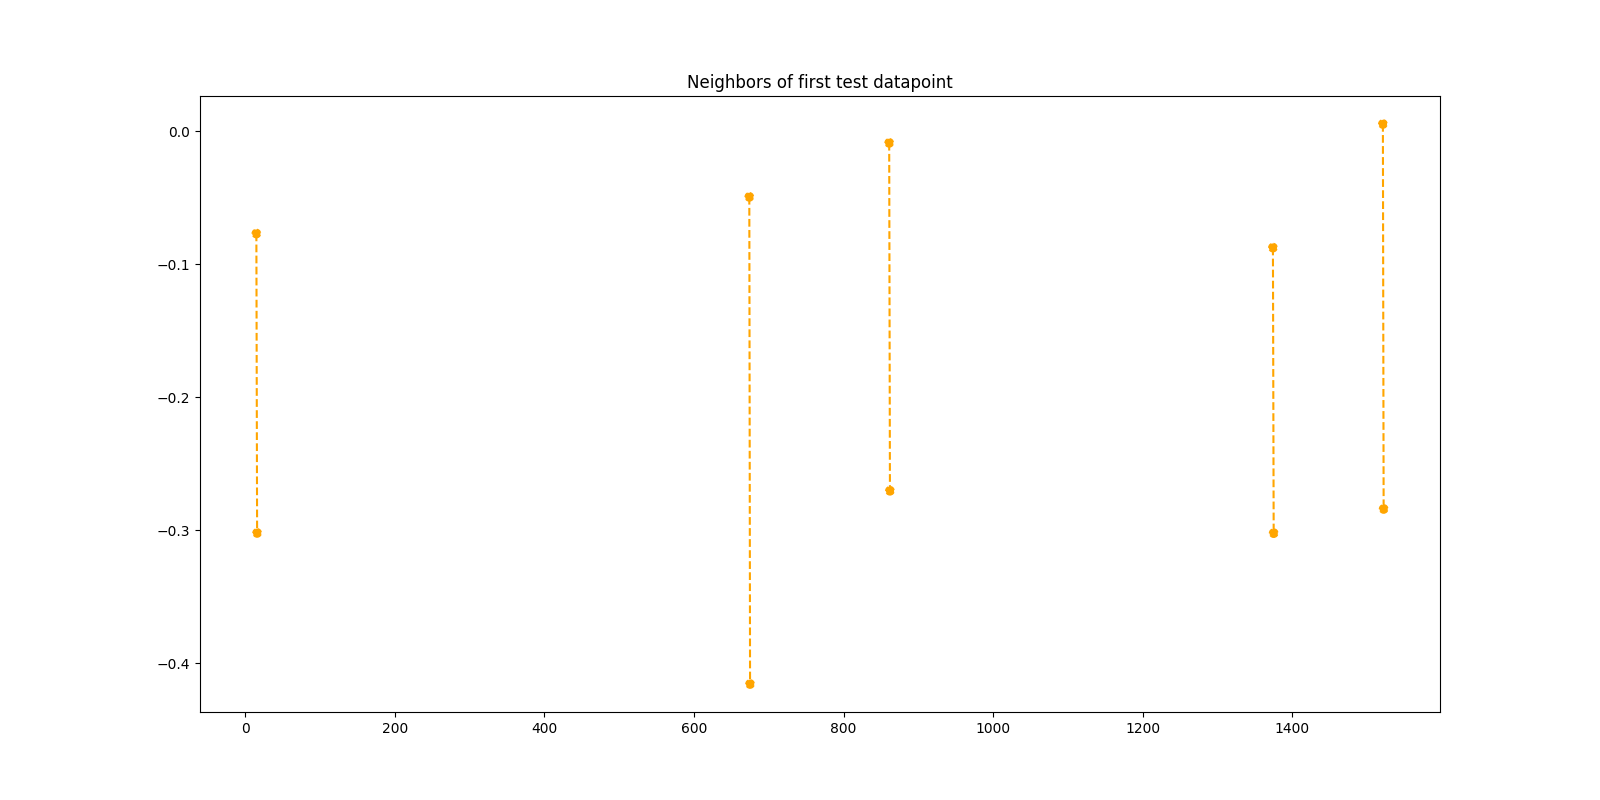
\includegraphics[width=0.40\textwidth]{Figures/AirportNonLin/Neighbors of first test datapoint.png}
    \caption{Neighbors of First Test Datapoint.}
    \label{ndata}
\end{figure}

\begin{figure}[ht]
    \centering
    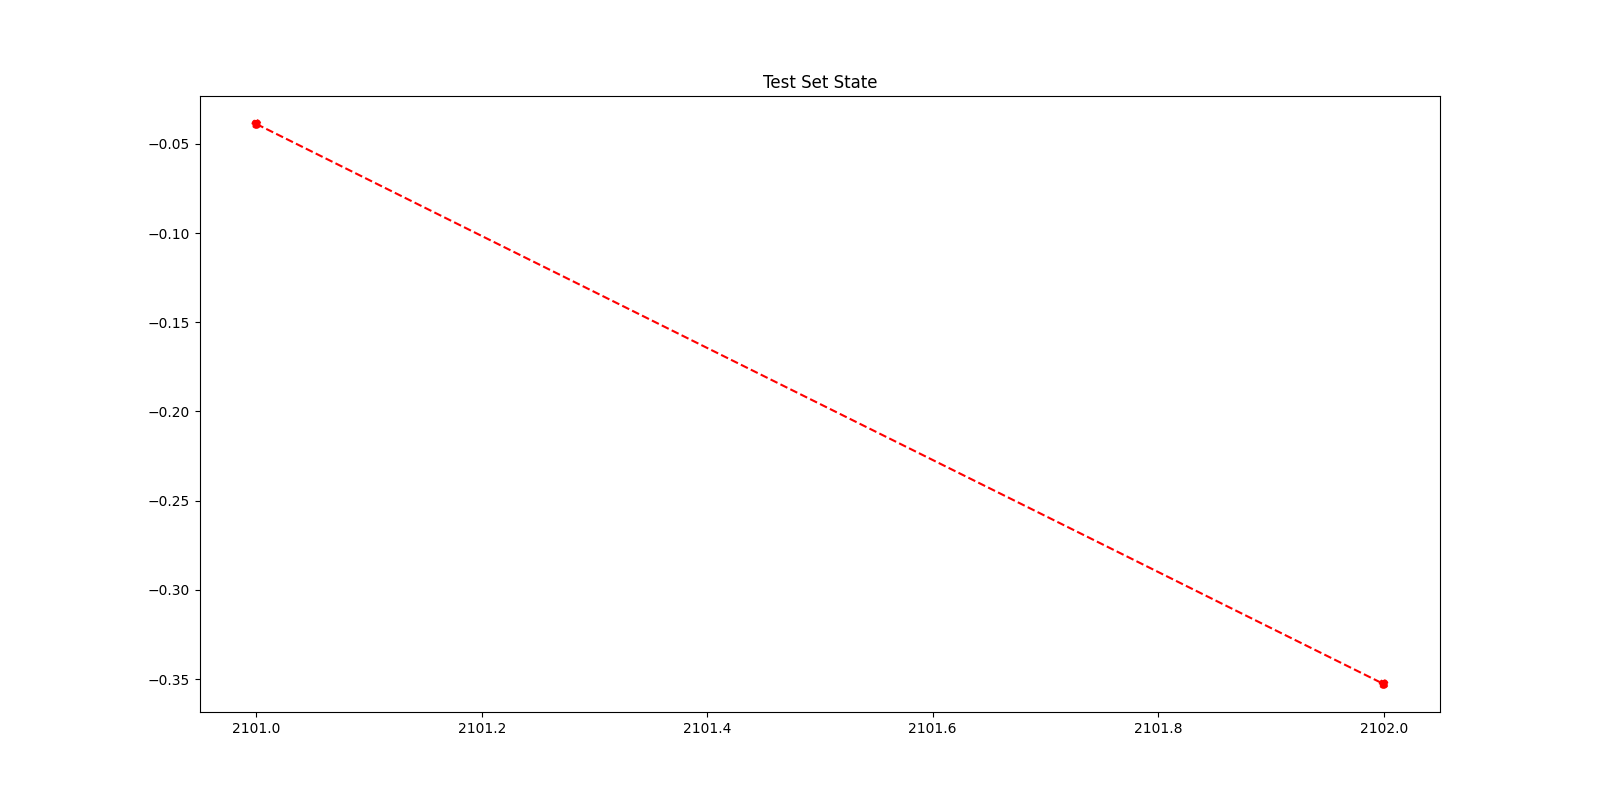
\includegraphics[width=0.40\textwidth]{Figures/AirportNonLin/Test Set State.png}
    \caption{Test Set State.}
    \label{TESTA}
\end{figure}
\vspace{80mm}

\begin{figure}[ht]
    \centering
    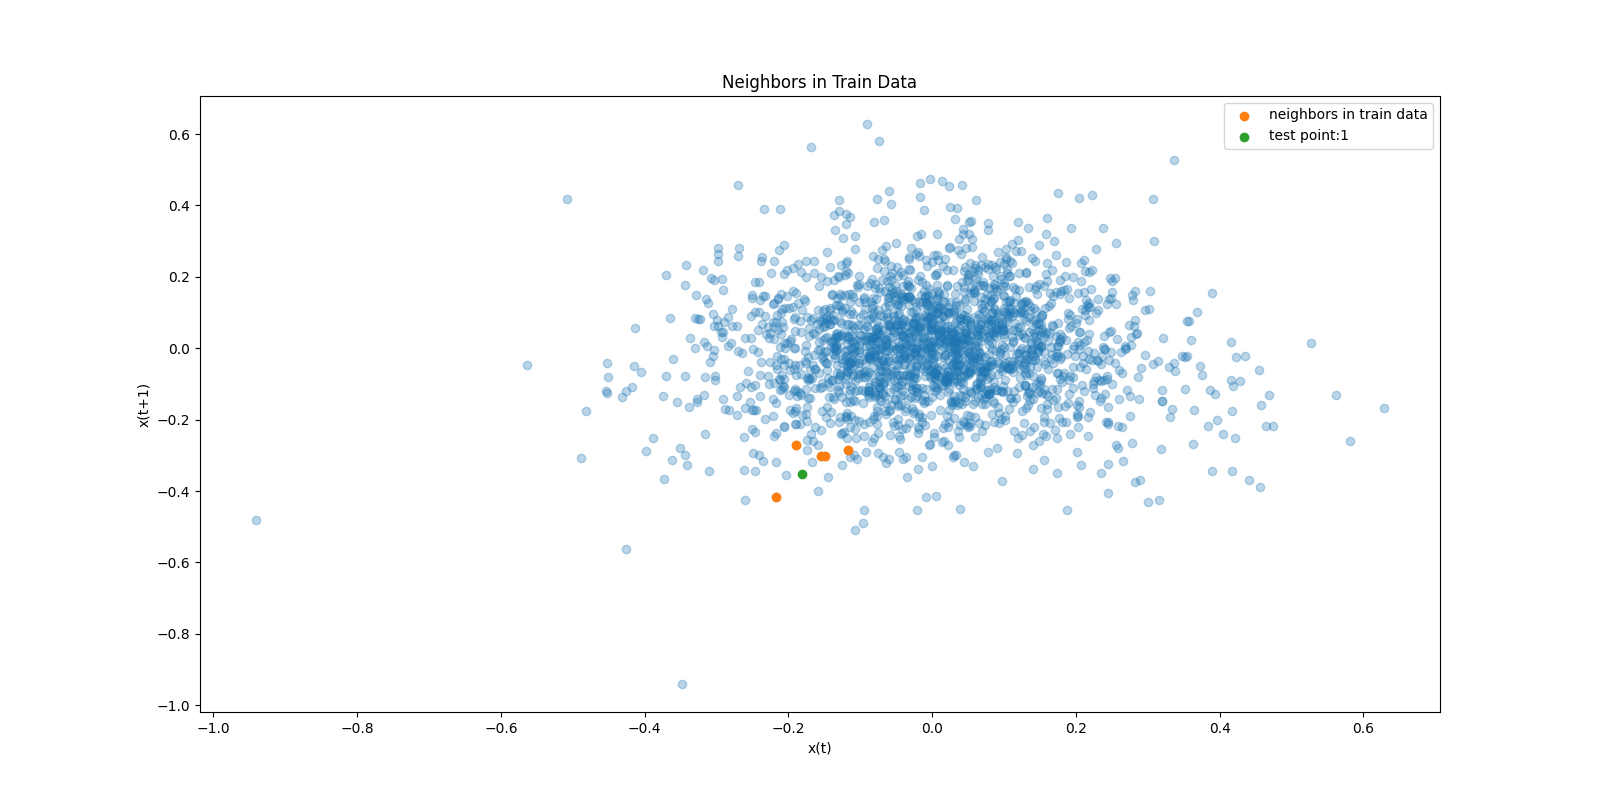
\includegraphics[width=0.40\textwidth]{Figures/AirportNonLin/Neighbors in Train Data.png}
    \caption{Neighbors in Train Data.}
    \label{traina}
\end{figure}

The LAP predictions are shown in Figure \ref{lapa}. We can see that they achieve high accuracy. The $NRMSE$ is very small (0.1256).

\begin{figure}[ht]
    \centering
    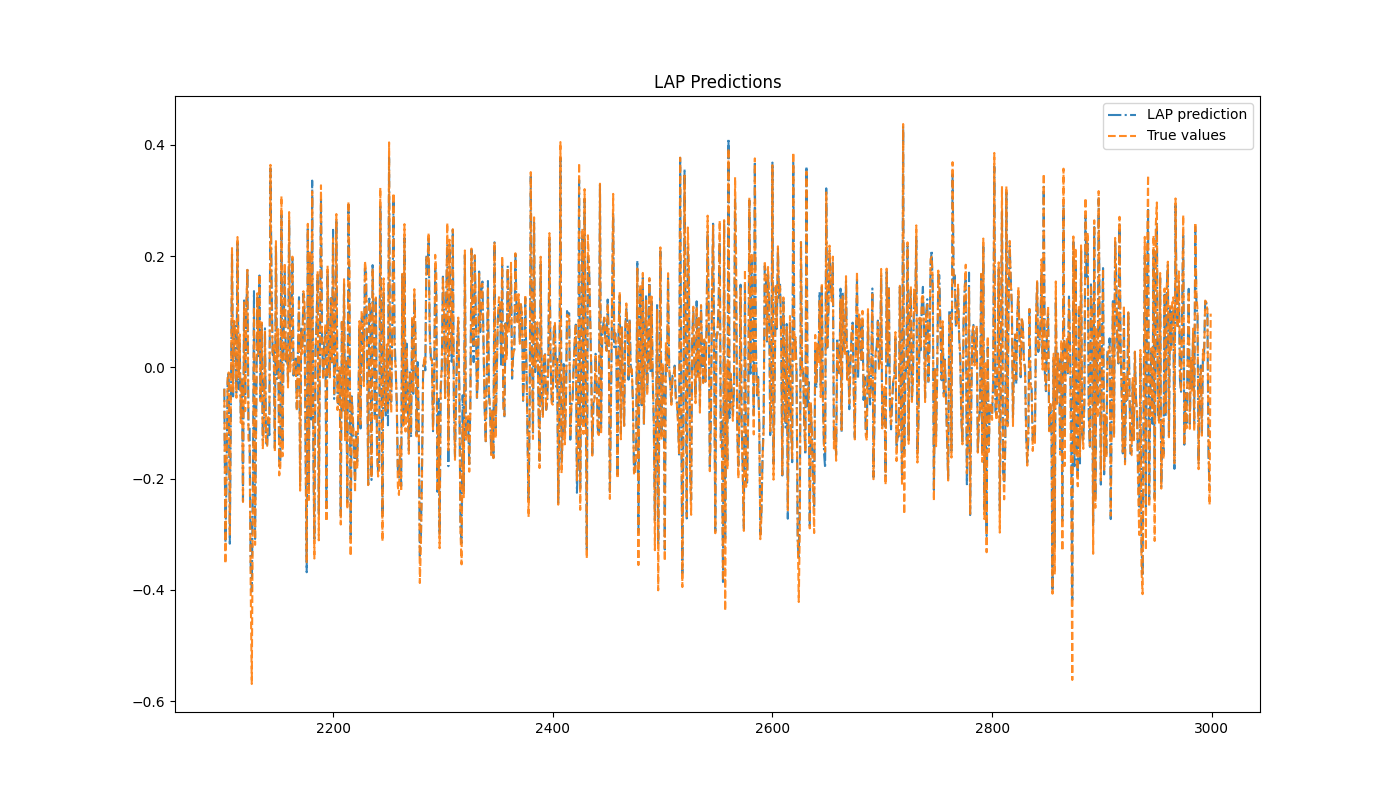
\includegraphics[width=0.45\textwidth]{Figures/AirportNonLin/LAP Predictions.png}
    \caption{LAP Predictions.}
    \label{lapa}
\end{figure}

Finally, the summary of OLS is shown in Figure \ref{tabla}. 

\begin{figure}[ht]
    \centering
    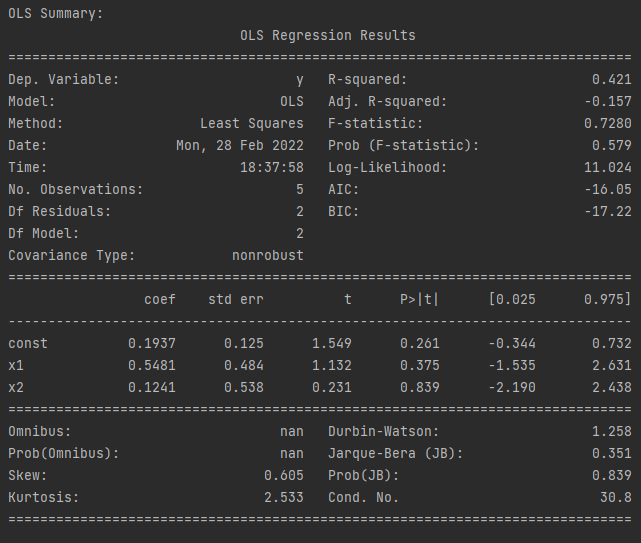
\includegraphics[width=0.35\textwidth]{Figures/AirportNonLin/olssummary.png}
    \caption{OLS Summary.}
    \label{tabla}
\end{figure}

%-Glasnevin-Average-Temperature-Linear-Analysis------------------------------------------------------------------
\section{Glasnevin Average Temperature \break Linear Analysis}

Now for the second region, Glasnevin, Figure \ref{tempg} and \ref{tempzoomg} show the Time Series of Daily Average Temperature during the past 60 years (1961-2021) and in increased resolution during 1998-2014 respectively. In Figure \ref{temphistg} the Histogram of the average temperatures is shown. It seems that the temperatures may be normally distributed, but we will not elaborate on that with any tests as well.

\begin{figure}[ht]
    \centering
    \includegraphics[scale=0.40]{Figures/GlasnevinLin/Average Temperature Time Series.png}
    \caption{Time Series of Daily Average Temperature in Glasnevin during the past 60 years (1961-2021).}
    \label{tempg}
\end{figure}

\begin{figure}[ht]
    \centering
    \includegraphics[scale=0.40]{Figures/GlasnevinLin/Average Temperature Histogram.png}
    \caption{Average Temperature Histogram.}
    \label{temphistg}
\end{figure}
\vspace{50mm}

\begin{figure}[ht]
    \centering
    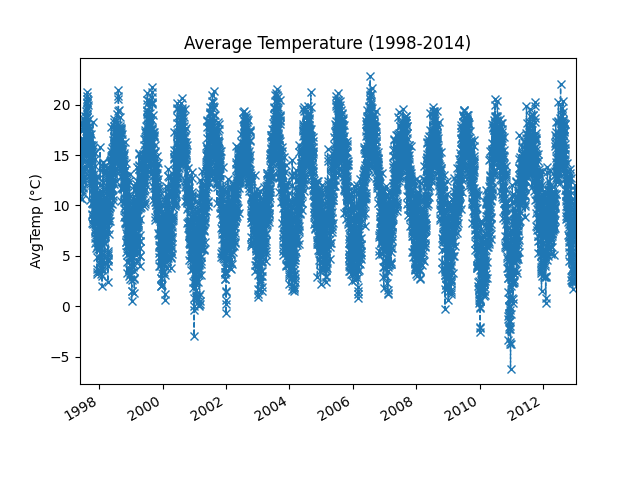
\includegraphics[scale=0.40]{Figures/GlasnevinLin/Average Temperature (1998-2014) Time Series.png}
    \caption{Time Series of Daily Average Temperature in Glasnevin during 1998-2014.}
    \label{tempzoomg}
\end{figure}

\subsection{Trend}

We begin the linear analysis of this time series also by exploring the trend. In this case, we notice in Figure \ref{tempzoomg} that the mean of $X_t$ is (slightly) changing in seemingly random ways. Also by looking at the yearly mean average temperature in Figure \ref{tempymg} we can see that the mean of average temperature is changing in stochastic ways from year to year. Furthermore by looking at the autocorrelation of $X_t$ in Figure \ref{tempcfg} we confirm that the time series is not stationary. We see that there is a significant correlation ($> 0.5$) between days for lag = $1$ to even lag = $40$. For these reasons we conclude that there exists a stochastic trend and we decide to eliminate it, because we believe it is produced by factors such as climate change, whereas we want to study the mechanism the temperature functions with and find the correlation between the values themselves. 

\begin{figure}[ht]
    \centering
    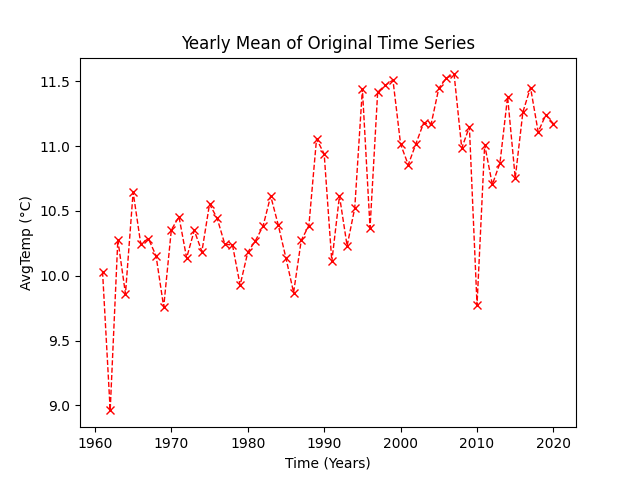
\includegraphics[width=0.45\textwidth]{Figures/GlasnevinLin/Yearly Mean of Original Time Series.png}
    \caption{Yearly Mean Average Temperature.}
    \label{tempymg}
\end{figure}

\begin{figure}[ht]
    \centering
    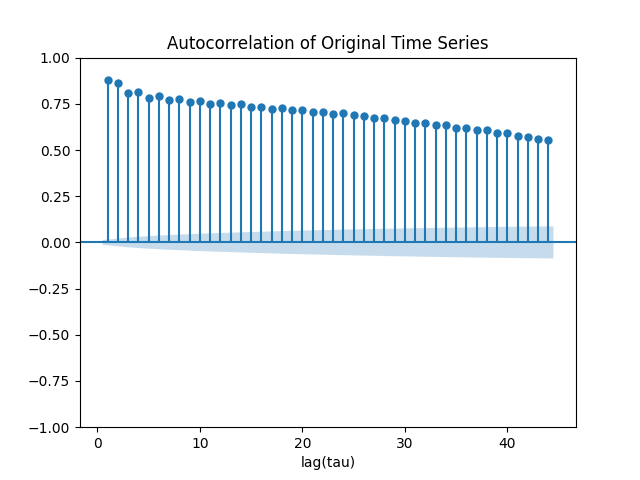
\includegraphics[width=0.45\textwidth]{Figures/GlasnevinLin/Autocorrelation of Original Time Series.png}
    \caption{Autocorrelation.}
    \label{tempcfg}
\end{figure}

Here we also studied three ways of detrending $X_t$. The first is estimating a polynomial (parametric) function to adapt to $X_t$ and a linear function with breakpoints to adapt to local consecutive parts of $X_t$. The degree of the polynomial we chose is $40$ and the number of breakpoints 160. The fits are demonstrated in Figure \ref{airpolbrg} in increased time resolution. The results in Figure \ref{airbrpolg} show that even a polynomial of degree 40 can not estimate the trend of $X_t$. The mean of the time series for both the polynomial and the linear piecewise breakpoint fit still displays variations with time. Proceeding with another way of detrending we created a moving average filter and then applying it (adapting it by taking the residuals) to $X_t$. The moving average filter we used with a window of 92 is shown in Figure \ref{airmag}.

\begin{figure}[ht]
    \centering
    \includegraphics[scale=0.4]{Figures/GlasnevinLin/Polynomial (40) and Breakpoint Fit (160).png}
    \caption{Polynomial Fit with degree $= 40$ and Linear Piecewise Fit with 160 breakpoints.}
    \label{airpolbrg}
\end{figure}

\begin{figure}[ht]
    \centering
    \includegraphics[scale=0.4]{Figures/GlasnevinLin/Polynomial (40) vs Breakpoint (160) Detrended.png}
    \caption{Detrending $X_t$ with the polynomial and breakpoint fit.}
    \label{airbrpolg}
\end{figure}
\vspace{80mm}

\begin{figure}[ht]
    \centering
    \includegraphics[scale=0.4]{Figures/GlasnevinLin/Moving Average (92).png}
    \caption{Moving Average Filter with a window of 92.}
    \label{airmag}
\end{figure}

Finally the last way of detrending is by obtaining the differences of logarithms of the time series by applying

\begin{equation}\label{diflogg}
    \begin{split}
        & X_t^{detrended} = \nabla sign(X_t)\log|X_t| \\
        & = sign(X_t)\log|X_t|-sign(X_{t-1})\log|X_{t-1}|.
    \end{split}
\end{equation}

In Figure \ref{airfdvsmag} we demonstrate the detrended time series resulting from adapting the moving average filter and applying the differences of logarithms. Judging from the figures, we concluded that it is best to detrend the time series using the moving average filter with window 92. 

\begin{figure}[ht]
    \centering
    \includegraphics[width=0.45\textwidth]{Figures/GlasnevinLin/Differences of Logarithms vs MA (92).png}
    \caption{Comparison of the detrended time series by adapting the moving average filter and by applying the differences of logarithms.}
    \label{airfdvsmag}
\end{figure}

\begin{table}
\begin{center}
\begin{tabular}{||c||c||c||} 
 \hline 
 Year & Means of $X_t$ & Means of $X_t^{detrended}$ \\ [0.5ex] 
 \hline\hline
 1961 & 10.03 & 0.08 \\ 
 \hline
 1971 & 10.35 & -0.00 \\
 \hline
 1981 & 9.93 & -0.005\\
 \hline
 1991 & 10.39 &  -0.02\\
 \hline
 2001 & 11.42 &  -0.009\\
 \hline
 2011 & 11.53 &  -0.005\\
 \hline
 2021 & 10.75 &  0.075\\
 \hline
\end{tabular}
\end{center}
\caption{Yearly Means of original and Detrended\break Average Temperature Time Series.}
\label{tablemg}
\end{table}

\subsection{Variance}

It is well known that by applying the logarithm to a time series the variance becomes invariant with time. We will check to see if this is applied to our case. In the previous section in Figure \ref{airfdvsmag} we proved that the trend becomes invariant with time by using the moving average filter. This is proved in Table \ref{tablemg} as the yearly means of the detrended time series are centered around zero with about $10^{-3}$ deviation which is trivial, they are practically zero. In the original time series there were clear mean fluctuations of 1 to 2 $^o C$ which is significant given that we measure temperature. 
\par The same methodology will be applied to check the variance. In Figure \ref{tempvg} the yearly variance of the original time series is shown. After using the moving average filter, the yearly variance has smaller fluctuations with time. The simplest solution we applied to make the variance invariant with time is use the logarithm of the positively shifted detrended time series to produce $X_t^{final}$. The exact transformation for every observation is

\begin{equation}\label{logmasg}
    \begin{split}
        & x_t^{final} = \log\left(x_t^{detrended}+\left|\min(X_t^{detrended})\right|+1\right).
    \end{split}
\end{equation}

The results are demonstrated in Table \ref{tablevg}. The variance is now practically zero for every year. Now after centering the time series, thus subtracting the mean from every observation, We also checked to see what happened to the trend when we applied the logarithm, and as shown in Table \ref{table1mg}, the mean for every year is invariant with time and centered at $0 ^o C$.

\begin{figure}[ht]
    \centering
    \includegraphics[width=0.45\textwidth]{Figures/GlasnevinLin/Yearly Variance of of Original Time Series.png}
    \caption{Yearly Variance of original Average Temperature Time Series.}
    \label{tempvg}
\end{figure}

\begin{table}
\begin{center}
\begin{tabular}{||c||c||c||c||} 
 \hline 
 Year & Variances of $X_t$ & \makecell{Variances of\\$X_t^{detrended}$} & \makecell{Variances of\\$\log X_t^{detrended}$} \\ [0.5ex] 
 \hline\hline
 1961 & 18.04 & 2.6 & 0.028\\ 
 \hline
 1968 & 18.33 & 3.1 & 0.035\\
 \hline
 1977 & 17.56 & 2.6 & 0.036\\
 \hline
 1995 & 27.84 & 4.3 & 0.052\\
 \hline
 2013 & 19.95 & 5.3 & 0.041\\
 \hline
 2021 & 18.45 & 6.6 & 0.033\\
 \hline
\end{tabular}
\end{center}
\caption{Yearly Variance of original, detrended and logarithm \break of detrended Average Temperature Time Series.}
\label{tablevg}
\end{table}

\begin{table}
\begin{center}
\begin{tabular}{||c||c||c||c||} 
 \hline 
 Year & \makecell{Mean of\\$\log X_t^{detrended}$} \\ [0.5ex]
 \hline\hline
 1961 & -0.00\\ 
 \hline
 1968 & 0.002\\
 \hline
 1977 & 0.0004\\
 \hline
 1986 & -0.002\\
 \hline
 1995 & -0.003\\
 \hline
 2004 & -0.002\\
 \hline
 2021 & 0.005\\
 \hline
\end{tabular}
\end{center}
\caption{Yearly Mean of logarithm of the detrended \break Average Temperature Time Series.}
\label{table1mg}
\end{table}

\subsection{Seasonality}

The initial time series in Figure \ref{tempzoomg} has an obvious seasonality. That makes sense because every year 
the same seasons come and go and this is basically the definition of seasons, with summer usually having the highest temperatures and winter the lowest. By looking at Figures \ref{logfing} and \ref{logfinzoomg} we see that by applying the moving of average filter of order 92 the seasonality is eliminated and this is still a fact when the logarithm is applied to the whole time series.

\begin{figure}[ht]
    \centering
    \includegraphics[width=0.45\textwidth]{Figures/GlasnevinLin/Logarithms of Detrended Average Temperature Time Series.png}
    \caption{Logarithms of Detrended Average Temperature Time Series.}
    \label{logfing}
\end{figure}

\begin{figure}[ht]
    \centering
    \includegraphics[width=0.45\textwidth]{Figures/GlasnevinLin/Logarithms of Detrended Time Series (Increased Resolution).png}
    \caption{Logarithms of Detrended Average Temperature Time Series (Increased Resolution).}
    \label{logfinzoomg}
\end{figure}

Now that we have eliminated the trend and seasonality and stabilized the variance of $X_t$ we can say that the time series is weakly stationary.

\subsection{Autocorrelation}

The autocorrelation of the detrended time series is shown in Figure \ref{airfddtg} for $\tau = 31$ lags with $95\%$ confidence intervals for significant correlations. We notice that there are significant correlations that decay exponentially and become insignificant after about $\tau = 7$ lags, which is to be expected given that we analyze temperature.

\begin{figure}[ht]
    \centering
    \includegraphics[width=0.45\textwidth]{Figures/GlasnevinLin/Autocorrelation of log(X_detrended).png}
    \caption{Autocorrelation for the final detrended time series for $\tau = 31$ lags.}
    \label{airfddtg}
\end{figure}

\subsection{Forecasting}

We will explore both the AR and Ma models for the time series, and also the ARMA. By calculating the partial autocorrelation we can see what $p$ to use for $AR(p)$. The partial autocorrelation is shown in Figure \ref{airfddtsg}. Also judging by the Akaike Information Criterion, we choose an AR model of order $4$ $(AR(4))$. The fit of this model, as well as the residuals, to the time series is shown in Figure \ref{ar4}.

\begin{figure}[ht]
    \centering
    \includegraphics[scale=0.2]{Figures/Partial Autocorrelation of log(X_detrended).png}
    \caption{Partial Autocorrelation for the final detrended time series for $\tau = 31$ lags.}
    \label{airfddtsg}
\end{figure}
\vspace{80mm}

\begin{figure}[ht]
    \centering
    \includegraphics[scale=0.2]{Figures/GlasnevinLin/ARIMA(4,0,0).png}
    \caption{AR(4) model fit to the the time series.}
    \label{ar4}
\end{figure}

The fitting error for T=10 is demonstrated in Figure \ref{fe4}. We can see that the AR(4) achieves a very good fit to the time series. The out of sample predictions of the model for time horizon T=36 and the rolling out of sample predictions for one year are shown in Figures \ref{hor4} and \ref{rol4}. We can see that the rolling predictions make a very good fit to the time series. By exploring the MA and ARMA models we get the results shown in Figures \ref{ma8} - \ref{rol33g}. The same procedure (AIC) was followed to select their orders. We can also see that the models MA(8) and ARMA(3,3) also achieve great fits. We chose MA(8) as our model-to-go, as we feel it expressed the temperature time series forecasts more accurately.
\vspace{80mm}

\begin{figure}[ht]
    \centering
    \includegraphics[width=0.45\textwidth]{Figures/GlasnevinLin/Fitting Error of ARIMA(4,0,0) for T = 10.png}
    \caption{AR(4) fitting error for T=10.}
    \label{fe4}
\end{figure}

\begin{figure}[ht]
    \centering
    \includegraphics[width=0.45\textwidth]{Figures/GlasnevinLin/AR(4) Out of Sample Predictions for Horizon T = 36.png}
    \caption{AR(4) Out of Sample Predictions for Horizon T = 36.}
    \label{hor4}
\end{figure}

\begin{figure}[ht]
    \centering
    \includegraphics[width=0.45\textwidth]{Figures/GlasnevinLin/AR(4) Rolling Out of Sample Predictions.png}
    \caption{AR(4) Rolling Out of Sample Predictions for one year.}
    \label{rol4}
\end{figure}
\vspace{80mm}

\begin{figure}[ht]
    \centering
    \includegraphics[width=0.45\textwidth]{Figures/GlasnevinLin/ARIMA(0,0,8).png}
    \caption{MA(8) model fit to the the time series.}
    \label{ma8}
\end{figure}

\begin{figure}[ht]
    \centering
    \includegraphics[width=0.45\textwidth]{Figures/GlasnevinLin/Fitting Error of ARIMA(0,0,8) for T = 10.png}
    \caption{MA(8) fitting error for T=10.}
    \label{fe8}
\end{figure}

\begin{figure}[ht]
    \centering
    \includegraphics[width=0.45\textwidth]{Figures/GlasnevinLin/MA(8) Out of Sample Predictions for Horizon T = 36.png}
    \caption{MA(8) Out of Sample Predictions for Horizon T = 36.}
    \label{hor8}
\end{figure}
\vspace{80mm}

\begin{figure}[ht]
    \centering
    \includegraphics[width=0.45\textwidth]{Figures/GlasnevinLin/MA(8) Rolling Out of Sample Predictions.png}
    \caption{MA(8) Rolling Out of Sample Predictions for one year.}
    \label{rol8}
\end{figure}

\begin{figure}[ht]
    \centering
    \includegraphics[width=0.45\textwidth]{Figures/GlasnevinLin/ARIMA(3,0,3).png}
    \caption{ARMA(3,3) model fit to the the time series.}
    \label{ma33g}
\end{figure}

\begin{figure}[ht]
    \centering
    \includegraphics[width=0.45\textwidth]{Figures/GlasnevinLin/Fitting Error of ARIMA(3,0,3) for T = 10.png}
    \caption{ARMA(3,3) fitting error for T=10.}
    \label{fe33g}
\end{figure}
\vspace{80mm}

\begin{figure}[ht]
    \centering
    \includegraphics[width=0.45\textwidth]{Figures/GlasnevinLin/ARMA(3,3) Out of Sample Predictions for Horizon T = 36.png}
    \caption{ARMA(3,3) Out of Sample Predictions for Horizon T = 36.}
    \label{hor33g}
\end{figure}

\begin{figure}[ht]
    \centering
    \includegraphics[width=0.45\textwidth]{Figures/GlasnevinLin/ARMA(3,3) Rolling Out of Sample Predictions.png}
    \caption{ARMA(3,3) Rolling Out of Sample Predictions for one year.}
    \label{rol33g}
\end{figure}

Finally, the Portmanteau tests were run for the three models, and we can see that all of them catch the linear correlations. The results are shown in Figures \ref{p4} - \ref{p33g}.
\vspace{80mm}

\begin{figure}[ht]
    \centering
    \includegraphics[width=0.40\textwidth]{Figures/GlasnevinLin/Ljung-Box Portmanteau Test for Residuals of ARIMA(4,0,0).png}
    \caption{Ljung-Box Portmanteau Test for Residuals of AR(4).}
    \label{p4}
\end{figure}

\begin{figure}[ht]
    \centering
    \includegraphics[width=0.40\textwidth]{Figures/GlasnevinLin/Ljung-Box Portmanteau Test for Residuals of ARIMA(0,0,8).png}
    \caption{Ljung-Box Portmanteau Test for Residuals of MA(8).}
    \label{p8}
\end{figure}

\begin{figure}[ht]
    \centering
    \includegraphics[width=0.40\textwidth]{Figures/GlasnevinLin/Ljung-Box Portmanteau Test for Residuals of ARIMA(3,0,3).png}
    \caption{Ljung-Box Portmanteau Test for Residuals of ARMA(3,3).}
    \label{p33g}
\end{figure}

%-Glasnevin-Average-Temperature-Non-Linear-Analysis--------------------------------------------------------------
\section{Glasnevin Average Temperature \break Non-Linear Analysis}

After testing the residuals (Figure \ref{resg}) of the stationary time series by applying th MA(8) model, we found out that they were white noise with the Portmanteau test (Figure \ref{portg}). So this the time series that we are going to apply non-linear analysis to. 

\begin{figure}[ht]
    \centering
    \includegraphics[width=0.45\textwidth]{Figures/GlasnevinNonLin/Residuals of MA(8).png}
    \caption{Residuals of selected MA(8) from Linear Analysis.}
    \label{resg}
\end{figure}

\begin{figure}[ht]
    \centering
    \includegraphics[width=0.45\textwidth]{Figures/GlasnevinNonLin/Ljung-Box Portmanteau Test for Residuals of ARIMA(0,0,8).png}
    \caption{Ljung-Box Portmanteau Test for Residuals of MA(8).}
    \label{portg}
\end{figure}

We created 40 new time series of the same length with the original residuals, without correlations, with random permutations. This was done to explore if there are any non-linear correlations. The residuals may be white noise, but are they iid, or have they non-linear correlations? To have non-linear correlations, a statistic must have a little difference in the original residuals in respect to the 40 time series. If a statistic is linear, then the estimated statistic of the original residual time series belongs in the distribution of the statistics from the 40 time series. The first statistic that we checked for is the Dickey-Fuller stationarity Statistical Test. If the p-value of the statistic is below the significance level, the zero hypothesis ($H_0$) is rejected and the time series is stationary.

\begin{figure}[ht]
    \centering
    \includegraphics[width=0.45\textwidth]{Figures/GlasnevinNonLin/Dickey-Fuller Test for Stationarity (if H0 rejected) on Original + 40 generated time series.png}
    \caption{Dickey-Fuller Test for Stationarity (if H0 rejected) on Original + 40 generated time series (y axis is scaled in $10^{-30}$).}
    \label{adfg}
\end{figure}

We can see in Figure \ref{adfg} that the zero hypothesis is rejected for the original residuals and all 40 randomly permutated time series. Subsequently, we explored the autocorrelation and the delayed mutual information for all 41 time series. The results are shown in Figures \ref{delg} and \ref{mig}. 
\vspace{80mm}

\begin{figure}[ht]
    \centering
    \includegraphics[width=0.45\textwidth]{Figures/GlasnevinNonLin/Delay estimation of original time series.png}
    \caption{Delay estimation of original time series.}
    \label{delg}
\end{figure}

\begin{figure}[ht]
    \centering
    \includegraphics[width=0.45\textwidth]{Figures/GlasnevinNonLin/Delay estimation of original + 40 time series.png}
    \caption{Delayed mutual information of original + 40 time series.}
    \label{mig}
\end{figure}

We can see that for all 41 time series the first minimum $\tau$ is one. Next we evaluated the dimension for the original and all sample time series, using the false nearest neighbors method. Figures \ref{dimg} and \ref{dimallg} demonstrate the results. We notice as well that the FNN belongs in the same distribution with the 40 time series. Moving on, the correlation sum is shown in Figures \ref{corsumg} and \ref{corlogg}.
\vspace{80mm}

\begin{figure}[ht]
    \centering
    \includegraphics[width=0.40\textwidth]{Figures/GlasnevinNonLin/FNN for original time series.png}
    \caption{False Nearest Neighbors for original time series.}
    \label{dimg}
\end{figure}

\begin{figure}[ht]
    \centering
    \includegraphics[width=0.40\textwidth]{Figures/GlasnevinNonLin/FNN for original + 40 time series.png}
    \caption{False Nearest Neighbors for original + 40 time series.}
    \label{dimallg}
\end{figure}

\begin{figure}[ht]
    \centering
    \includegraphics[width=0.40\textwidth]{Figures/GlasnevinNonLin/Local vs for original time series.png}
    \caption{Local $D_2$ vs $r$ for original time series.}
    \label{corsumg}
\end{figure}
\vspace{80mm}

\begin{figure}[ht]
    \centering
    \includegraphics[width=0.40\textwidth]{Figures/GlasnevinNonLin/log(r), log(C(r)).png}
    \caption{log(r) log(C(r)).}
    \label{corlogg}
\end{figure}

Next, for embedding dimension $m = 3$ (we did no choose $m = 4$ for visualization ) and $\tau = 1$ the plotted 3D Attractor is shown in Figure \ref{attg}. The attractor shape is like a cloud, implying that there is not any non-linear correlation in the time series. This was also made clear before, as the statistics that we estimated all belong to the same distribution. 

\begin{figure}[ht]
    \centering
    \includegraphics[width=0.45\textwidth]{Figures/GlasnevinNonLin/3D Attractor of Residual Time Series (tau=1).png}
    \caption{3D Attractor of Residual Time Series (tau=1).}
    \label{attg}
\end{figure}

So here we explored the predictions with LAP and LLP. Firstly, the train and test set is shown in Figure \ref{trg}. After embedding the train and test sets in dimension 3 and $\tau = 1$, we used the KDTree. 

\begin{figure}[ht]
    \centering
    \includegraphics[width=0.45\textwidth]{Figures/GlasnevinNonLin/Train and Test Set.png}
    \caption{Train and Test Sets.}
    \label{trg}
\end{figure}

The neighbors of the first test datapoint are demonstrated in Figure \ref{ndatg}, the Test Set State is shown in Figure \ref{TESTg}, and the neighbors of the first test datapoint in train data are shown in Figure \ref{traing}.

\begin{figure}[ht]
    \centering
    \includegraphics[width=0.45\textwidth]{Figures/GlasnevinNonLin/Neighbors of first test datapoint.png}
    \caption{Neighbors of First Test Datapoint.}
    \label{ndatg}
\end{figure}

\begin{figure}[ht]
    \centering
    \includegraphics[width=0.45\textwidth]{Figures/GlasnevinNonLin/Test Set State.png}
    \caption{Test Set State.}
    \label{TESTg}
\end{figure}
\vspace{80mm}

\begin{figure}[ht]
    \centering
    \includegraphics[width=0.45\textwidth]{Figures/GlasnevinNonLin/Neighbors in Train Data.png}
    \caption{Neighbors in Train Data.}
    \label{traing}
\end{figure}

The LAP predictions are shown in Figure \ref{lapg}. We can see that they achieve high accuracy. The $NRMSE$ is very small (0.132). Finally, the summary of OLS is shown in Figure \ref{tablg}. 
\vspace{80mm}

\begin{figure}[ht]
    \centering
    \includegraphics[width=0.45\textwidth]{Figures/GlasnevinNonLin/LAP Predictions.png}
    \caption{LAP Predictions.}
    \label{lapg}
\end{figure}

\begin{figure}[ht]
    \centering
    \includegraphics[width=0.35\textwidth]{Figures/GlasnevinNonLin/olsum.png}
    \caption{OLS Summary.}
    \label{tablg}
\end{figure}

%-Conclusion-----------------------------------------------------------------------------------------------------
\section{Conclusion}

In conclusion, the main difference is that we used an AR(6) model for the Dublin Airport Time Series and an MA(8) model for the Glasnevin Time Series. Overall the temperature time series seems to behave linearly in both regions, with the observations in one day being related to the temperatures of one to six days before, which is to be expected. As for the non-linear analysis, no non-linear correlations were found, implying that the system behind temperature is not dynamic.

\end{document}